% Chapter 1

\chapter{Quark-Gluon Plasma} % Main chapter title
\label{Chapter1} % For referencing the chapter elsewhere, use \ref{Chapter1} 

\section{Strongly interacting matter}
\label{sec:Intro}
A deep insight into the matter which constituted the universe and its evolution
starting from few second after the Big Bang has been achieved so far, in the past and recent years.
From the decoupling of neutrinos 
and the nucleosynthesis, the evolution of the Universe is today quite well
understood. Still, we have very little knowledge on what happened before.
In the early Universe, after 10 $\mu$s after the Big Bang, matter was in a state very far away from the one described by Quantum 
Chromodynamics (QCD) at temperatures and energy densities 
of ordinary nuclear and hadronic matter. 
In QCD, the effective coupling between quarks 
and gluons depends on the squared transverse momentum $q^2$ exchanged
 in the interaction. In one loop calculation, the following relation for the
 strong coupling constant $\alpha_s$ can be found~\cite{Wilson:1970ag}:
\begin{equation}
\alpha_s(q^2)=\frac{\alpha_s (\mu^2)}{1+\alpha_s (\mu^2) \frac{33-2n_f}{12\pi}ln(\frac{-q^2}{\mu^2})}
\end{equation}
where $\mu$ is the momentum scale and $n_f$ is the number of flavors 
considered. When exploring regions with $|q^2|\rightarrow$ 0, which also 
correspond to distances larger than 1 fermi (hadron size), the strong 
coupling constant $\alpha_s$ becomes large. On the other hand, the coupling 
decreases with increasing $q^2$. This is the so-called {\it asymptotic freedom}, 
a general feature of non-Abelian gauge theories. Hence, interactions between 
quarks and gluons become weaker as their mutual distance decreases or as the 
exchanged momentum increases.
Consequently, matter at very high temperatures or energy densities (or at high values 
of both of them) undergoes a phase transition from a state with quarks confined into 
hadrons into a new state of matter with on-shell quarks and gluons free to move over
volumes larger than the hadron size. This deconfined state is called Quark-Gluon Plasma (QGP).
In the primordial universe, quarks and gluons were expected to be in this plasma state, their interaction 
being dominated by the strong fundamental force.
The temperature of the Universe at the time of the QGP 
was of hundreds of MeV.
Right after some tens of microseconds, the cooling of this state down to 
a temperature $T \sim$ 150 MeV (that corresponds to $\sim 10^{10}$ K: to give an idea, the temperature inside the Sun is 
around 11$\times 10^{6}$ K) lead to the 
creation of structures, irreversibly binding quarks together, inside colorless
hadrons. The QCD matter phase diagram (Fig.~\ref{fig:QCDphase}) predicts the 
strongly-interacting matter to occur in different phases, depending on the 
temperature T and the baryo-chemical potential $\mu_{B}$. \footnote{The baryo-chemical potential $\mu_{B}$ is defined as 
the energy needed to increase by one unit the net baryon number, 
$\mu_{B}$ = $\partial$E/$\partial N_B$, thus being directly related to the baryonic density.} 
At low temperatures and for $\mu_{B} \sim 1$ GeV we are in the situation of the 
ordinary nuclei. By compressing or heating nuclear matter a state of 
hadronic gas is reached, nucleons can interact elastically and form resonances and other hadrons. 
At extremely high values of temperature and energy density a transition to the Quark-Gluon 
Plasma is expected. These were the conditions of the primordial universe in the
first micro-seconds after the Big Bang.
The experimental research of this phase of matter started in the second half of the `80s, 
with the first fixed target experiments at the Super Proton Synchrotron (SPS) at CERN and at the Alternating Gradient Synchrotron (AGS) at 
Brookhaven National Laboratory (BNL). For the first time scientists tried to 
reproduce in the laboratory such a state of matter, initially through acceleration 
of light nuclei (Si and S respectively), then moving to heavier nuclei (Pb and Au).\\


\begin{figure}[h!]
\centering
 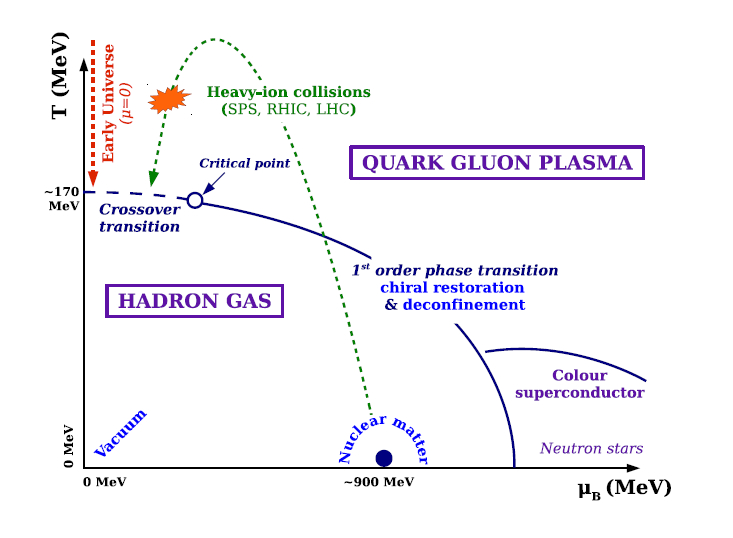
\includegraphics[width=0.8\textwidth] {FigCap1/QCDphase.jpeg}
\caption{Phase diagram of strongly interacting matter.}
\label{fig:QCDphase}
\end{figure}

Although the transformations in the early universe concerned the interactions among quarks,
this phase transition would have never happened if not driven by macroscopic
conditions, like the system temperature and energy density. The comprehension 
of the evolution of this state of matter 
has the promise to become accessible if we understand the thermodynamics 
laws of the QCD. It is not obvious indeed, nevertheless intriguing, 
to understand whether the QCD thermodynamics applies to the fireball 
created in the heavy-ion collisions in the laboratory, and whether the 
emitted hadrons keep a trace of the thermodynamics processes. \\

After the SPS, the Relativistic Heavy-Ion Collider (RHIC) at BNL 
has conducted experiments to create hot QCD matter through Au-Au 
collisions with the highest collision energy $\sNN = 200$ GeV per nucleon-nucleon
collision, one order of magnitude above the top of SPS energy. 
The Large Hadron Collider (LHC) at CERN is conducting experiments 
along the same line with the highest achievable centre-of-mass 
energy of $\sNN = 5.02$ TeV per nucleon-nucleon collision.

\section{Micro bang vs big bang: timescales of expansion, baryonic number}
\label{sec:Timescales}
The system created in the laboratory by colliding
relativistic nuclei presents many similarities with 
the matter of the primordial universe, but also some differences. 
A Hubble-like expansion drives the 
evolution of the system after the collisions in the laboratory and the fireball undergoes different phases (see Fig.~\ref{fig:timescales}): 
\begin{itemize}
\item Pre-equilibrium phase: parton scatterings produce a large number of partons; 
they interact among each other leading the fireball to thermalise after a 
time of $\sim$ 0.6-1 fm/c;
% with the creation of high-$\pt$ probes (heavy quarks, photons) and low-$\pt$ particles;
\item QGP phase: with high-energy collisions, if the temperature inside the fireball 
exceeds the critical temperature $T_{\rm c}$, the system is in a deconfined 
phase with partonic degrees of freedom. While the phase of QGP in the early universe lasted
tens of microseconds, due to the interplay of gravity and
radiative pressure of the expanding matter, the plasma created in the laboratory 
has a lifetime of the order of 10$^{-23}$ seconds. During this time, it rapidly expands
and cools down, thus the size and local properties of
the fireball change rapidly, contrary to what happened in the 
early universe.

\item Hadronisation phase: while expanding, the temperature 
of the medium drops down and, when the critical temperature $T_{\rm c}$
is reached, quarks and gluons give rise to hadrons (confinement); the hadron
gas continues the expansion and the temperature lowers further.

\item Chemical freeze-out: inelastic processes cease and the relative abundances of the various hadron species are fixed;
\item Kinetic freeze-out: even elastic collisions finish, fixing the momentum distribution of the produced particles. 
\end{itemize} 

\begin{figure}[h!]
\centering
 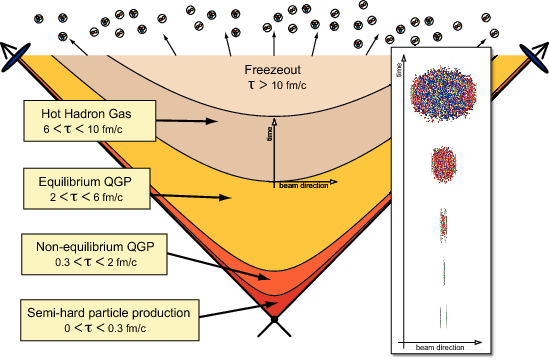
\includegraphics[width=0.8\textwidth] {FigCap1/timescales.png}
\caption{The space-time evolution of a heavy-ion collision~\cite{Strickland:2014pga}. }
\label{fig:timescales}
\end{figure}


Unlike in the early universe, we expect in the laboratory a significant matter-antimatter 
asymmetry in the particle abundance, at the lower centre-of-mass energies due to the
stopping of the colliding nucleons. 
At the energies of AGS and SPS, colliding nuclei tend to stop each other, forming a 
dense, baryon-rich matter and hence a system with a large $\mu_{B}$. At higher 
energies ($\sNN > 100 \Gevc$), they pass through each other leaving a nearly 
baryon-free matter in the region at central rapidity. In this case the system is closer 
to the conditions of zero baryo-chemical potential of the primordial universe. 
RHIC experiments were the first to enter in the  ``baryon free'' domain. Today, ALICE, 
CMS and ATLAS, thanks to unprecedentedly high energy beams at the LHC, are 
exploring this region with even smaller baryo-chemical potential. 
Figure~\ref{fig:YieldsVsEnergyAndronic} shows the measured yields of identified 
particles and anti-particles at mid-rapidity \footnote{The rapidity $y$ is defined as 
\mbox{$y = 1/2 \; {\rm ln}((E+p_{L})/(E-p_{L}))$}, where $E$ is the particle energy 
and $p_{L}$ its momentum longitudinal to the beam direction} as a function of the 
centre-of-mass energy of the collision, covering results by experiments at the 
AGS, SPS, RHIC and LHC~\cite{Andronic:2014zha}. The difference in the production 
of p and $\bar{\rm p}$ at low energies is a clear example of what discussed above. 
Because of the large stopping power in the low-$\sNN$ region, the quark content of
 the fireball is dominated by the quark content of the colliding nucleons. At LHC 
 energies, yields of particles and anti-particles are the same, 
 indicating the increasing transparency in the collision. 
The difference in the production of $\pi^+$ and $\pi^-$ at low $\sNN$ is due to the 
isospin composition of the fireball. Finally, the difference between $K^+$ and $K^-$ 
and between $\Lambda$ and $\bar{\Lambda}$ is again due to their quark content, 
$K^+ (u\bar{s})$, $K^- (\bar{u}s)$, $\Lambda (uds)$, $\bar{\Lambda} (\bar
{u}\bar{d}\bar{s})$: like in the proton case, the quark content of the colliding nucleons
drives the fireball content, in regimes of large stopping power. When the collision energies become 
high enough so that the we enter the ``baryon free'' domain and particle-to-antiparticle ratios $\approx$ 1,
the baryo-chemical potential approaches $\approx 0$ values.


\begin{figure}[!t]
  \centering
  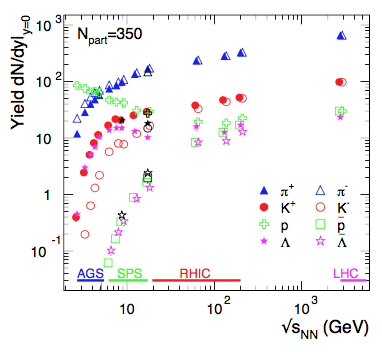
\includegraphics[width=8.5cm]{FigCap1/YieldsVsEnergyAndronic.png}
  \caption{Collision energy dependence of the multiplicities (yield, dN/dy, at mid-rapidity) of pions, kaons, protons and lambda hyperons and their antiparticles, measured in central collisions (corresponding to an average number of 350 participant nucleons in the collision) of Au or Pb nuclei~\cite{Andronic:2014zha}.}
  \label{fig:YieldsVsEnergyAndronic}
\end{figure}

% /* Expansion rates differ by 18 orders of magnitude
% Expansion in 3d, not 4d; driven by pressure gradients, not gravity
% Time scales measured in fm/c rather than billions of years
% % Distances measured in fm rather than light years
% “Heavy-Ion Standard Model” still under constructio
% Similarities: Hubble-like expansion, expansion-driven dynamical freeze-out
% chemical freeze-out (nucleo-/hadrosynthesis) before thermal freeze-out
% (CMB, hadron pT -spectra)
% initial-state quantum fluctuations imprinted on final state*/
\section{What theory tells us}
\label{sec:Lattice}
QCD is the widely accepted theory for the strong interaction. 
Phenomena at high energies, or equivalently, very short distances can be
predicted via a perturbative approach, since the coupling constant is weak. 
How the quarks are bound in the hadrons, however, is controlled by 
the large-scale behaviour of the coupling, which increases with distance. 
For such reason, lattice calculation is an indispensable technique. 
Lattice QCD is a non-perturbative treatment of QCD formulated 
on a discrete grid or lattice of points in space and time~\cite{Philipsen:2012nu}. 
Because of the non-perturbative nature of the theory, 
numerical simulations of Lattice QCD are the only tool 
allowing for calculations from first principles. The discretisation of the 
space-time continuum provides two main 
advantages: on one hand the problem of ultraviolet divergences typical 
of the perturbative approach is solved 
as the step of the lattice defines the shortest distance scale and hence a 
cut-off value for the momentum scale. 
On the other hand, we wish to describe a system of particles in a finite 
volume $V$, which is in thermal contact 
with a heat bath at temperature $T$. Associated with the particles, there 
may be a set of conserved charges 
$N_i$, with \textit{i}=1, 2, ... (such as the particle number, electric charge, 
baryon number etc.). In quantum field 
theory, the most direct description is in terms of the grand canonical ensemble, 
defining a density operator $\rho$ and a partition function $Z$ of the system at a temperature $T$:
\begin{equation}
\rho =e^{-\frac{1}{T}(H-\mu_iN_i)},\quad Z=Tr(e^{-\frac{1}{T}(H-\mu_iN_i)})=  \int dx \langle x|e^{-\frac{1}{T}(H-\mu_iN_i)}|x\rangle,
\end{equation}
where $\mu_i$ are the chemical potentials for the conserved charges, and 
the quantum mechanical trace is a sum over 
all energy eigenstates $|x\rangle$ of the Hamiltonian H. 
From the partition function, all other thermodynamic equilibrium quantities are 
calculable. The basic idea behind lattice 
QCD is the possibility to express the grand canonical partition function using the 
path integral representation, going in the 
domain of imaginary time. Actually, the partition function has a very similar 
formulation to the propagator of a quantum 
mechanical system between two space-time points $\langle x_b|e^{-iH(t_b-t_a)}|x_a\rangle$. 
The path integral 
formulation allows the use of Monte-Carlo methods to find the equilibrium states of the system. 
With lattice discretisation, some ``order parameters'' can be defined, which are 
sensitive to certain processes and accessible from lattice calculations. From them, 
estimates of characteristics parameters, like the critical temperature $T_c$ for the transition
to a deconfined state, can be obtained. Among the order parameters, there are:
\begin{figure}[!t]
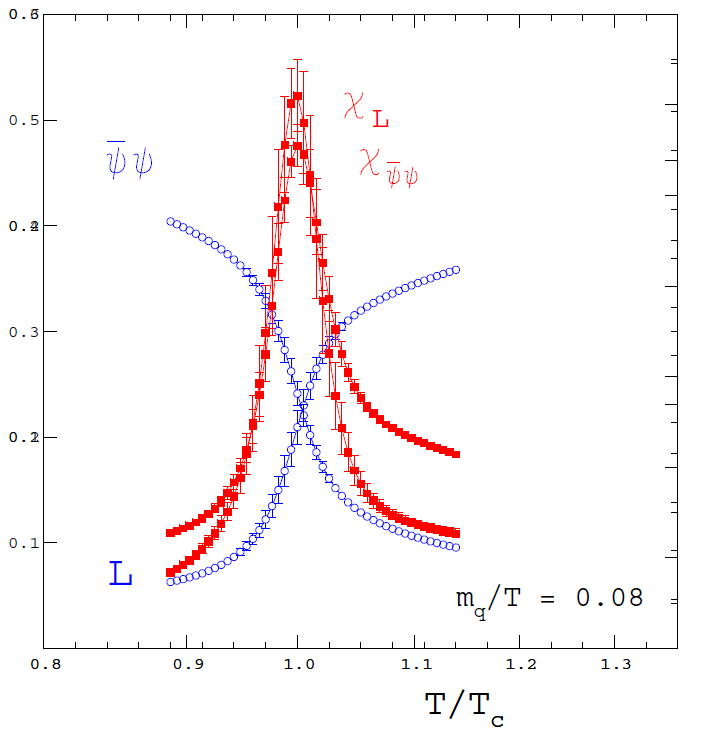
\includegraphics[width=6cm,height=6cm]{FigCap1/Lattice1.png} 
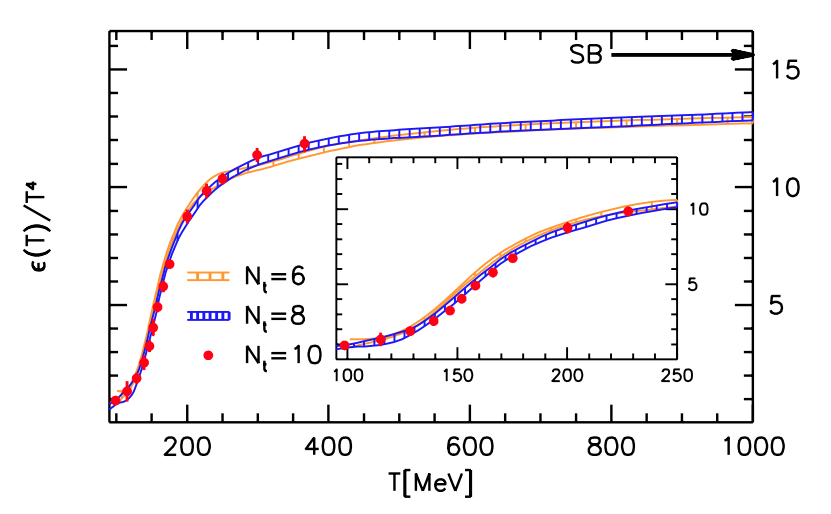
\includegraphics[width=7.5cm,height=5.8cm]{FigCap1/BW_EnDensity.png}
 \caption{(Left) Chiral condensate $\langle \bar{\psi}\psi\rangle$ and free energy function L (blue) as function of temperature. Their susceptibilities are shown in red~\cite{Karsch:2001vs}. (Right) Lattice simulation of energy density as a function of temperature. The arrows indicate the position of the Stefan-Boltzmann limit~\cite{Borsanyi:2010cj}.}
\label{fig:Lattice}
\end{figure}

\begin{itemize}
\item \textbf{Polyakov loop,} defined as:
\begin{equation}
L(T)\sim {\rm exp}\{-V(r)/T\},
\end{equation}
where $V(r)$ is the potential between a static quark-antiquark pair separated by a distance $r$. 
In pure gauge theory $V(r)\sim \sigma r$ where $\sigma$ is the string tension \footnote{Two colour sources 
in a confining gauge theory are bound together by a thin flux tube and this hypothesis is the
core of the effective string description of confinement~\cite{Caselle:2002vq}.}; hence V($\infty$) = $\infty$, 
and $L = 0$. In a deconfined medium, colour screening among the gluons leads to a melting of the 
string, which makes $V(r)$ finite at large $r$; hence $L$ does not vanish. It thus 
becomes a parameter for estimating the state of deconfinement. 
Fig.~\ref{fig:Lattice} (left) shows lattice results for $L(T)$ and the 
corresponding susceptibility $\chi_L(T)\sim \langle T^2 \rangle - \langle T \rangle ^2$. 
\item \textbf{Chiral condensate: }the effective quark mass is measured by the expectation value 
of the corresponding term in the Lagrangian, $\langle  \bar{\psi}\psi\rangle (T)$. 
The chiral symmetry is the invariance of the Lagrangian under an axial transformation of the fermion field:
\begin{equation}
\Psi \rightarrow e^{-i \gamma_{5} \frac{\vec{\tau} \cdot \vec{\theta}}{2}}\Psi
\end{equation}
where $\vec{\tau}$ are the three Pauli matrices and $\gamma_5$ 
is the chiral operator. In the limit of 
vanishing current quark masses, the Lagrangian becomes 
chirally symmetric. When confined into 
hadrons, the bare quarks ``dress'' themselves with gluons acquiring 
an effective constituent mass. 
After the transition to a deconfined phase, the quarks 
would recover the ``bare'' mass, and the 
chiral symmetry should be approximately restored. In the calculations, 
the order parameter for the transition is the effective 
quark mass, measured as the expectation value of the corresponding 
term in the Lagrangian, that is the 
chiral condensate $\langle \overline{\psi}\psi \rangle$. In Fig.~\ref{fig:Lattice} 
(left) the behaviour of 
the order parameter as a function of temperature is shown. 
Recent results provide a measure of the critical temperature 
$T_c$ from the results for the chiral condensate, 
and it is estimated as $T_c = (154 \pm 9) $ MeV~\cite{Petreczky:2012rq}.
\item \textbf{Energy density $\epsilon$} at deconfinement: 
in Fig.~\ref{fig:Lattice} (right) it 
can be seen that $\epsilon/T^4$ changes quickly at the critical temperature 
$T_c$, increasing from a low 
value typical of an hadron gas to a higher value closer to what expected 
for an ideal gas in the Stefan-Boltzmann limit of 
massless quarks and gluons. N$_{\rm t}$ is the number of points in the temporal
direction of a hyper-cubic lattice~\cite{Borsanyi:2010cj}. The 
remarkable deviation of $\epsilon/T^4$ from the
Stefan-Boltzmann limit is a clear signal of surviving
correlations in the deconfined phase.
The rapid increase in energy density is expected to occur as consequence of the increased number of degrees of 
freedom in the phase transition. %Recent calculations of Lattice QCD predicts as critical temperature $ \sim 160$ MeV~\cite{Karsch:2001vs}.

\end{itemize}


\begin{figure}[!b]
  \centering
  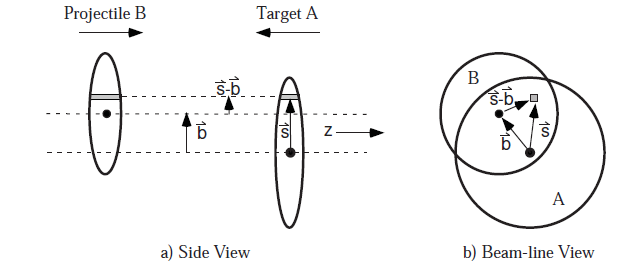
\includegraphics[width=12cm]{FigCap1/glauber.png}
  \caption{Schematic view of a nucleus-nucleus collision described in terms of the impact parameter $b$ in the longitudinal (left) and transverse (right) plane.}
  \label{fig:image10}
\end{figure}

\section{Collision Geometry and the Glauber Model}
\label{sec:glauber}
In a collision of two nuclei, the impact parameter \textit{b}, i.e. the distance 
between the centres of the nuclei in the transverse plane of the collision, can 
span values from 0 to about $R_1+R_2$, where  $R_1$ and  $R_2$ are the radii of 
the two nuclei if approximated with hard spheres. 
Small values of $b$ ($\lesssim$ 3.5 fm) imply central collisions. 
The impact parameter can not be measured directly, yet it is 
possible to relate it to observables like the multiplicity of particles produced in the 
collision, the transverse 
energy or the number of spectator nucleons. 
The Glauber model is used to calculate the geometrical quantities that 
characterise the collision (such as the number of nucleons participating in the collisions,
the number of spectator nucleons), and that can be correlated with some
observables (such as multiplicity, transverse energy) to estimate the centrality of the
collision~\cite{Miller:2007ri}.
The model provides a phenomenological description assuming that the nucleus-nucleus 
collision can be treated as a superposition of independent nucleon-nucleon collisions.
Under the assumptions (optical limit) that, (i) at sufficiently high energies, the nucleons 
inside the nuclei are essentially undeflected after the collision, (ii) the
 nucleons are independent in the nucleus, (iii) protons and neutrons 
 are indistinguishable and (iv) the radius of the nucleus is large compared 
 to the extent of the nucleon-nucleon force, we can define the thickness 
 functions of nuclei A, B for a certain value of impact parameter $b$ (see Fig.~\ref{fig:image10}):
\begin{equation}
T_i(\vec s) = \int\,{\rm d}z \rho_i(\vec s,z).
\end{equation}
The thickness function is related to the nuclear density function $\rho$. The nuclear 
density is usually parameterised by a Woods-Saxon or 3-parameter Fermi distribution:
\begin{equation}
\rho (r) = \rho_0 \frac{1+w(r/R)^2}{1+{\rm exp}(\frac{r-R}{a})},
\end{equation}
where $\rho_0$ is the nuclear density in the center of the nucleus, 
$R = (6.62 \pm 0.06)$ fm is the radius parameter of the ${}^{208}$Pb, 
$a = (0.546 \pm 0.010)$ fm is the skin thickness of the Pb nucleus and $w$ 
characterizes deviations from a spherical shape ($w=0$ for Pb). 
The nuclear overlap function is then defined as:
\begin{equation}
T_{\rm AB} (\vec{b}) = \int \,{\rm d}^2s T_A(\vec s)T_B(\vec s - \vec b)
\end{equation}
and it gives the probability for two incoming nucleons inside two nuclei colliding 
with impact parameter \textit{b} to be in the same elementary area ${\rm d}^2s$ in the transverse plane.
By considering the mean of a binomial distribution, the average number of 
binary nucleon-nucleon collisions $\langle N_{\rm coll}\rangle$ as a function 
of the impact parameter \textit{b} can then be written as~\cite{Miller:2007ri}:
\begin{equation}
\langle N_{\rm coll}\rangle = AB \times T_{\rm AB}(b)\; \sigma^{\rm inel}_{\rm NN},
\end{equation}
where $A$ and $B$ are the mass numbers of the colliding nuclei and $\sigma^{\rm inel}_{\rm NN}$
is the inelastic interaction cross-section of the two nucleons.
The average number of participant nucleons in the collisions (nucleons of target 
and projectile that interact) can be obtained as a function of the impact parameter $b$ as:
\begin{equation}
\begin{aligned}
N_{\rm part} (b) &= \int A \; T_A(\vec{s}) [1- (1-  \sigma^{\rm inel}_{\rm NN} T_B(\vec{b}-\vec{s}))^B]{\rm d}^2s \\
& + \int B \; T_B(\vec{b}-\vec{s}) [1- (1-  \sigma^{\rm inel}_{\rm NN} T_A(\vec{s}))^A]{\rm d}^2s.
\end{aligned}
\end{equation}
The inelastic cross-section for a collision between two nuclei (A and B), 
in a certain centrality range ($0 < b < b_c$) 
can be expressed using the Glauber model geometry, as:
\begin{equation}
\label{eq:sigmaABGlauber}
\sigma_{AB}(b_c) = \int_0^{b_c} 2\pi b\,{\rm d}b [1 - (1 - \sigma^{\rm inel}_{\rm NN}T_{\rm AB}(b))^{AB}]. %\simeq \int_0^{b_c} 2\pi b\,db \cdot AB\cdot T_{\rm AB}(b)  \sigma^{\rm inel}_{\rm NN}.
\end{equation}
\begin{figure}[!t]
\centering
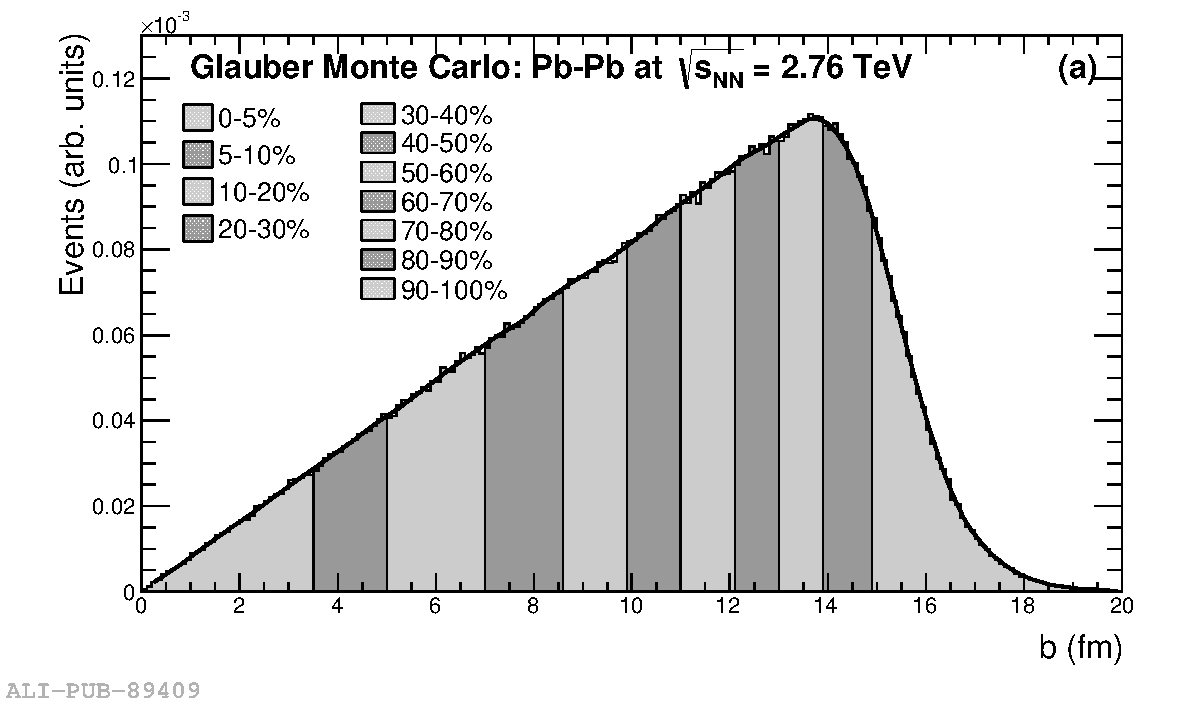
\includegraphics[width=7cm]{FigCap1/Glauberimpactpar.pdf}
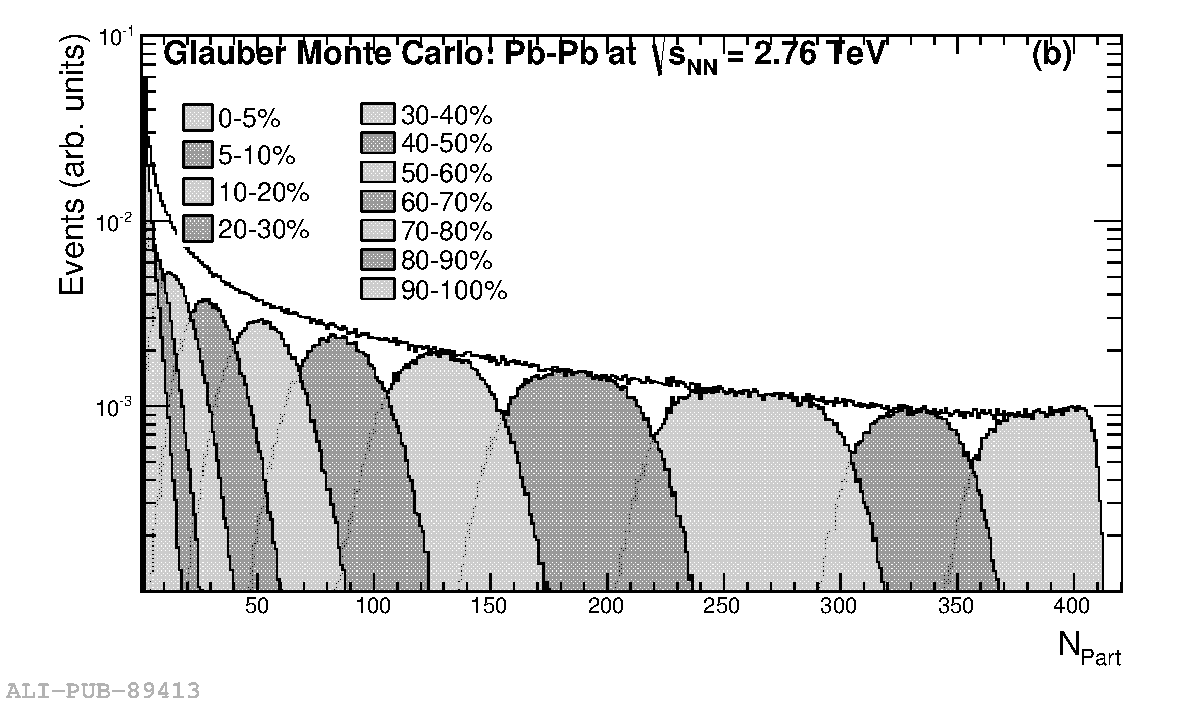
\includegraphics[width=7cm]{FigCap1/GlauberNpart.pdf}
\caption{Left: impact parameter distribution obtained from Glauber MC simulations for Pb-Pb collisions at $\sNN = 2.76$ TeV. Right: the corresponding $N_{\rm part}$ distributions for different intervals of centrality percentiles.}
\label{fig:glaubMC}
\end{figure}
The centrality is usually expressed in terms of percentiles of the total nuclear 
interaction cross section $\sigma_{AB}$ in Eq.~\ref{eq:sigmaABGlauber}.
The percentile of the cross-section for collisions in a given impact parameter
interval $b_{min}< b <b_{max}$ (see Fig.~\ref{fig:glaubMC}) is given by:
\begin{equation}
c=\frac{1}{\sigma_{AB}}\int_{b_{min}}^{b_{max}} \frac{{\rm d}\sigma_{AB}}{{\rm d}b'}{\rm d}b'.
\end{equation}
A simple approach to use the Glauber Model formulation for the
 calculation of geometry related quantities like $N_{\rm part}$ and $N_{\rm coll}$
is a Monte Carlo implementation. 
Furthermore, it is possible to simulate experimental quantities 
like the charged particle multiplicity and to apply centrality cuts similar to those used in the analysis of real data. 
In the simulation the nucleon distribution in the two colliding nuclei is randomly generated
according to their nuclear density distributions.
A random impact parameter $b$ is also associated to the collision according to the distribution
d$\sigma$/d$b \propto 2\pi b$. The nucleons travel along straight-line
trajectories and the inelastic nucleon-nucleon cross-section is assumed to be independent
of the number of collisions a nucleon underwent before. A nucleon-nucleon collision takes place if
their distance $d$ in the plane orthogonal to the beam axis satisfies the following condition:
\begin{equation}
d \leq \sqrt{\sigma^{\rm inel}_{\rm NN}/\pi}.
\end{equation}
Optical Glauber and MC Glauber show good agreement when calculating 
simple geometric quantities like $N_{\rm part}$ and $N_{\rm coll}$ as
a function of impact parameter. Some discrepancies appear at the highest values of the impact parameter.
This is mainly due to the fact that in the Optical Approximation the incoming nucleon sees the incoming nucleus as a smooth density object and does not account for event-by-event density fluctuations~\cite{Miller:2007ri}.



In Chapter 3, more details will be given about the calculation 
of N\textsubscript{part} and N\textsubscript{coll} and about the centrality 
determination in the ALICE experiment.


\section{Heavy-ion physics at the LHC}
\label{sec:HIatLHC}
The SPS program, with its several experiments, 
was mainly aimed at understanding whether a new state of matter, with the 
characteristics of a Quark-Gluon Plasma, could actually be created in the laboratory.
For a more quantitative study of the properties of this
system, we had to wait for the following experiment era, at the RHIC and LHC colliders.
However, the first results from the SPS revealed that Pb-Pb collisions 
were not simply a trivial superposition of elementary proton-proton (pp) collisions.
First of all, it was possible to measure quantitatively
the energy density and temperature of the fireball formed after collisions of two Pb nuclei.
A formula derived by Bjorken~\cite{Bjorken} 
revealed the energy density of the system to be around
3 GeV/fm$^{3}$, slightly above the phase transition
predicted by the Lattice QCD at about 0.5-0.6 GeV/fm$^3$~\cite{Hands}. At that energy density,
Lattice QCD gives a plasma temperature of about 210 MeV. The main experimental observations at the SPS 
showed an abundant production of hadrons
containing strange quarks~\cite{Sandor:2004bg} (``strangeness enhancement"), 
the reduced production of the J/$\psi$ mesons~\cite{Abreu:2000ni} 
(``anomalous J/$\psi$ suppression") and the yields of 
low-mass lepton pairs~\cite{Damjanovic:2005ni} (``$\rho$ melting"). They constituted 
the signals that a new state of matter had been found.
Moreover, the NA49 experiment gave the first indications that the fireball medium 
could be described by QCD hydrodynamics, with the measurement
of the elliptic flow of pion and proton in semi-peripheral Pb-Pb collisions 
at top SPS energy~\cite{Alt:2003ab}. This observable, described in more detail 
in Sec.~\ref{sec:AnisotropicFlow}, is related with the
initial spatial anisotropy of the overlapping area of the two colliding nuclei, that is 
then converted into a final momenta anisotropy. Such a process is only possible 
if the fireball is guided by collective motion effects in a liquid-like medium with  
small viscosity. The initial results from RICH confirmed the picture 
of an extremely strongly interacting and almost perfect liquid QGP, enough opaque 
to quench any fast parton travelling through it.\\
This effect and the experimental observations mentioned before will 
have a deeper insight in the LHC research program. In the following, a revision of some of the most 
important results and open points regarding heavy-ion physics at the higher LHC energies
is reported. 

\begin{figure}[!t]
  \centering
  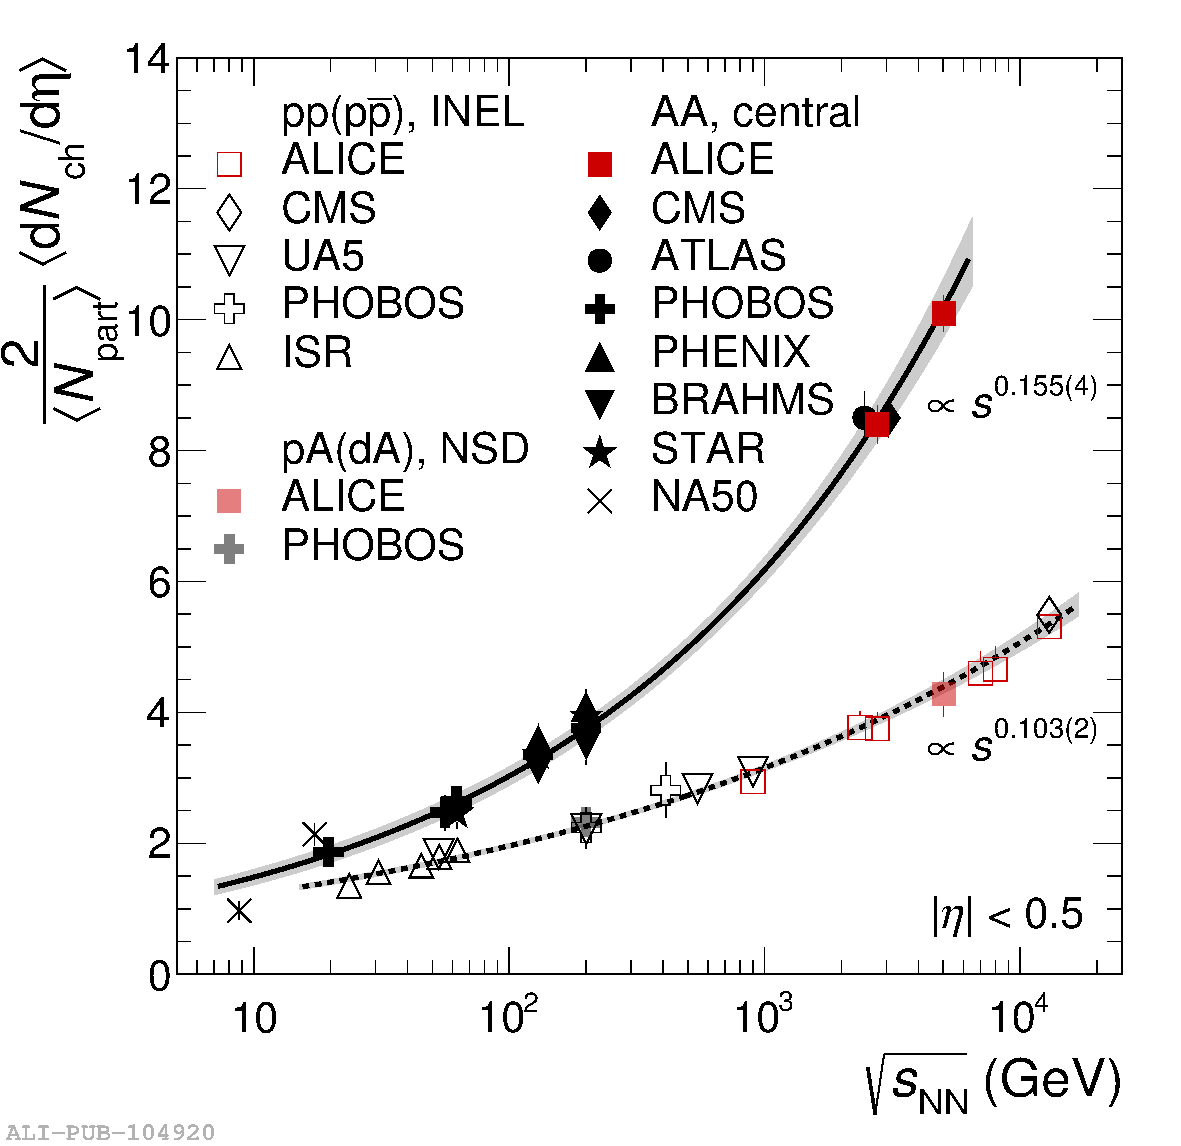
\includegraphics[width=7cm]{FigCap1/dNchdEtaVsEnergy.pdf}
  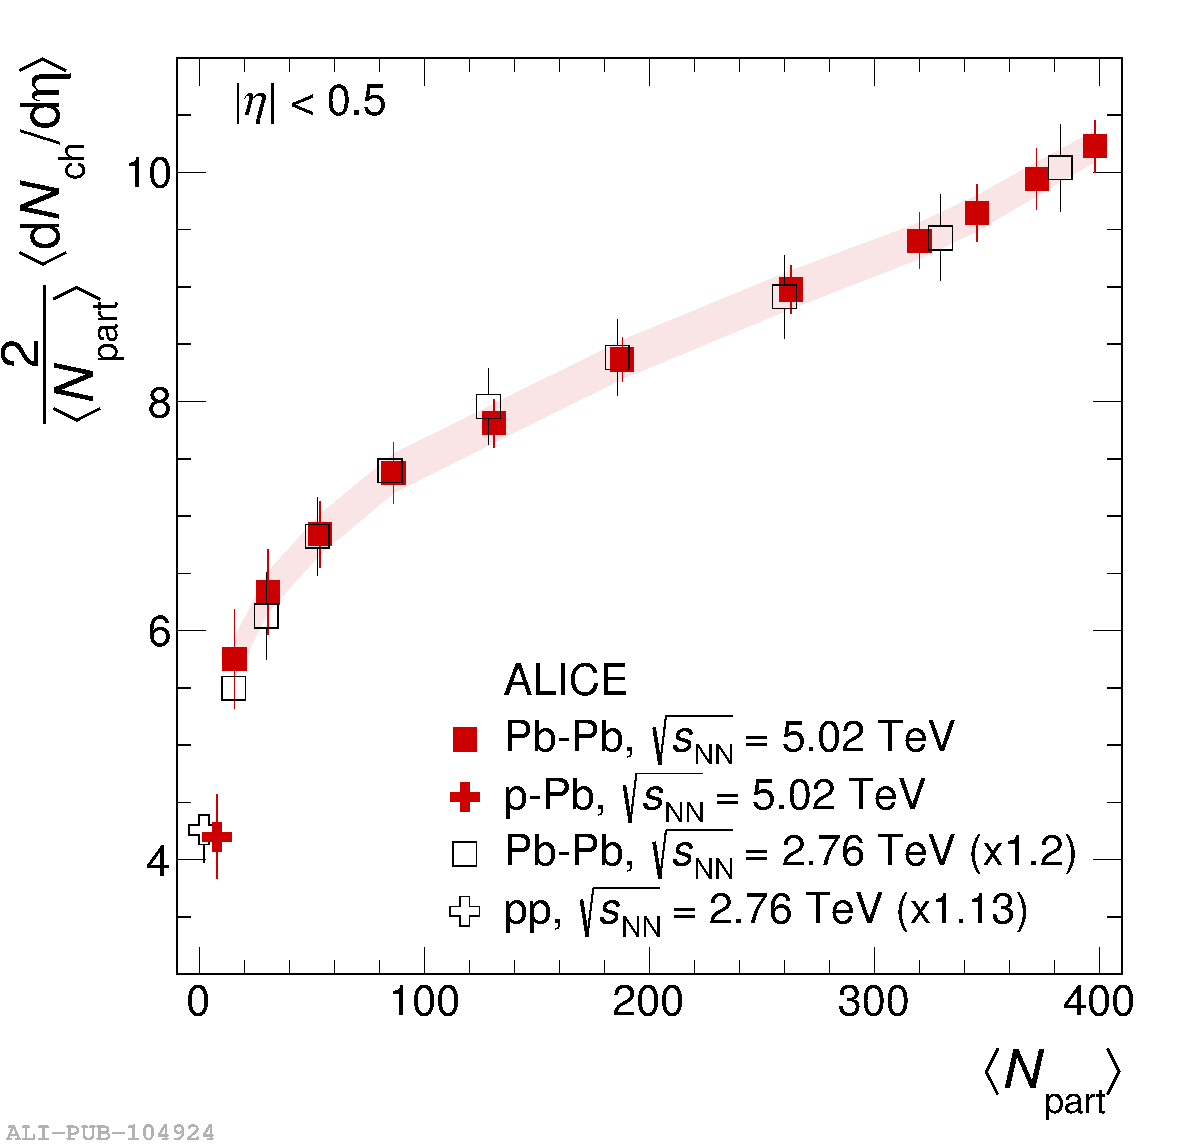
\includegraphics[width=7cm]{FigCap1/dNchdEtaVsNpart.pdf}
  \caption{(Left) Charged particle pseudo-rapidity density per participant pair for pp and central AA collisions as a function of centre-of-mass energy per nucleon pair, measured in different colliding systems~\cite{Adam:2015ptt}. The fit to the power law is shown as solid (A-A) and dashed (pp) lines, together with the uncertainties on the dependence (shaded bands). (Right) Centrality dependence of (d$\Nch$/d$\eta$)/($\langle N_{\rm part} \rangle/2$) for p-Pb and Pb-Pb collisions at $\sNN=5.02$ TeV~\cite{ALICE:2012xs,Adam:2015gka}, Pb-Pb collisions at $\sNN=2.76$ TeV~\cite{Aamodt:2010cz} and pp collisions at $\sqrt{s}=7$ TeV measured with ALICE.}
  \label{fig:dNchdEta}
\end{figure}

\subsection{Particle multiplicity and energy density}
\label{sec:partMult}
The number of particles produced in the collision (multiplicity) is related to the 
density of the created medium. In fact particle multiplicity depends both on the 
centrality and on the energy of the collision. This observable is usually presented as 
a pseudo-rapidity ($\eta = - {\rm ln}(\tan(\theta/2))$ density of charged particles at 
mid-rapidity (d$\Nch$/d$\eta |_{\eta=0}$). This is useful to compare experimental 
results with different acceptances. Furthermore, particle density is usually 
divided by the average number of nucleon pairs participating to the collision 
($\langle N_{\rm part}\rangle$/2), to compare results of different 
colliding systems. The measurements by ALICE in the 5\% 
most central Pb-Pb collisions at $\sNN = 5.02$ TeV showed a density of charged 
particles at mid-rapidity $\langle $d$\Nch$/d$\eta \rangle = 1943 \pm 54$ 
and, normalised per participant pair, (d$\Nch$/d$\eta$)/($\langle N_{\rm part} \rangle/2$) $ 
= 10.1 \pm 0.3$~\cite{Adam:2015ptt}.  
The left panel of Fig.~\ref{fig:dNchdEta} presents (d$\Nch$/d$\eta$)/($\langle N_{\rm part} \rangle/2$) 
as a function of the centre-of-mass energy per nucleon pair. The energy dependence 
of the charged multiplicity for central heavy-ion collisions can be fitted with a power 
law of the form $as^b$, where $b = 0.155 \pm$ 0.004~\cite{Adam:2015ptt}. 
The rise is much stronger than in pp collisions where $b = 0.103 \pm 0.002$, 
obtained from a fit to the same function. It can also be noticed that the values 
of (d$\Nch$/d$\eta$)/($\langle N_{\rm part} \rangle/2$) from p-Pb collisions are included in the figure 
and lay on the pp curve, showing that the strong rise in A-A collisions is not 
only due to the multiple interactions undergone by the participating nucleons, 
present in p-A collisions as well. The right panel of Fig.~\ref{fig:dNchdEta} 
shows the values of (d$\Nch$/d$\eta$)/($\langle N_{\rm part} \rangle/2$) 
as a function of the average number of participant nucleons 
measured by ALICE in p-Pb~\cite{ALICE:2012xs} and Pb-Pb~\cite{Adam:2015ptt} 
collisions at $\sNN = 5.02$ TeV. The Pb-Pb measurements at 
$\sNN = 2.76 $ TeV~\cite{Aamodt:2010cz} are also shown, scaled by a 
factor of 1.2 (calculated from the observed $s^{0.155}$ dependence), as 
well as the pp measurements at $\sqrt{s}= 7$ TeV~\cite{Adam:2015gka} 
scaled by a factor of 1.13. The charged particle density per participant pair 
shows a strong dependence on $\langle N_{\rm part}\rangle$, decreasing 
by a factor of about 1.8 from most central collisions to peripheral ones. The 
measurement of particle production per participant pair can be used to 
constrain models describing particle production in heavy-ion collisions 
with different mechanisms. Among the others, theoretical calculations 
 based on gluon saturation can give a good description of data
 (rcBK-MC~\cite{Albacete:2011fw}, Kharzeev, Levin and Nardi~\cite{Kharzeev:2004if} 
 and Armesto, Salgado and Wiedemann~\cite{Armesto:2004ud}). These models assume the existence of a
 transverse momentum scale at which the gluon and quark phase space 
 density saturates, thus limiting the number of produced partons and, 
 hence, of particles.
 This results also in a centrality dependence of the multiplicity of 
 heavy-ion collisions in the models, as observed in the experimental
data. \\
The simplified Bjorken model~\cite{Bjorken:1982qr} can be used to 
estimate the initial spatial energy density from the measured 
$\langle$d$\Nch$/d$\eta$$\rangle$:
\begin{equation}
\label{Bjorken}
\epsilon_{Bj} = \frac{\langle m_T\rangle}{\tau_f A}\frac{{\rm d}N_{\rm ch}}{{\rm d}y}
\end{equation}
where $\tau_f$ is the formation time of the secondary particles, A is the overlap 
area of the two colliding nuclei, $\langle m_T \rangle$ is the average transverse 
mass of the created particles defined as $m_{\rm T} = \sqrt{m^{2}+\pt^2}$ and $y$ 
is the rapidity. Starting from the measured values of d$\Nch$/d$\eta$, it is 
possible to estimate the energy density of the medium created in the collision.
At top RICH energy (200 GeV), for the most central collisions, one obtains 
$\sim 5$ GeV/fm$^3$ at the conservative estimate for the formation time 
$\tau_f$ = 1 fm/c~\cite{Bjorken:1982qr}, well above the critical value predicted 
by lattice QCD for the phase transition to QGP. For central Pb-Pb collisions at the LHC 
at $\sNN$ = 2.76 TeV the value of $\epsilon_{Bj}$ is much higher and is 
around $\sim 14$ GeV/fm$^3$~\cite{Chatrchyan:2012mb}.

\subsection{Hadron multiplicities and chemical freeze-out}
\label{sec:chemFO}
If we assume that a chemical and thermal equilibrium governs the medium when it
 undergoes chemical freeze-out, the thermal nature of the medium 
 should be imprinted in the final hadron abundances. 
 If these conditions occur, the behavior of the system at the 
 equilibrium can be described via a statistical approach, using a description 
 of the final particle yields in terms of thermodynamical quantities. 
 Following the approach described in~\cite{BraunMunzinger:2003zd}, 
 we can introduce the partition function Z($T,V,\mu_{Q}$), that 
 allows for a quantitative description of the statistical properties 
 of the equilibrated system, as a function of temperature $T$, 
 volume $V$ and chemical potentials $\mu_{Q}$. 
\begin{figure}[!ht]
  \centering
  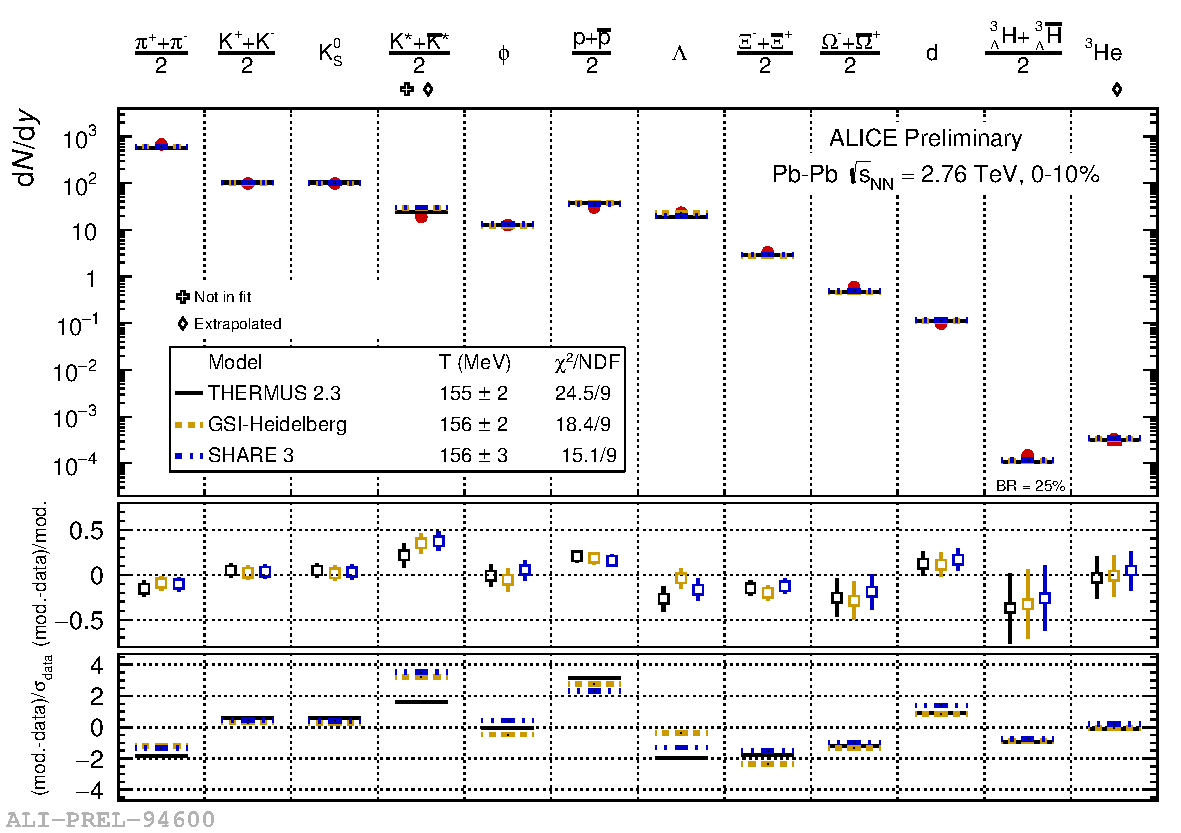
\includegraphics[width=12cm]{FigCap1/GCThermalFit_PbPb010.pdf}
  \caption{Grand Canonical thermal fit to ALICE 0-10\% Pb-Pb data at $\sqrt{s_{\rm NN}} = 2.76$ TeV~\cite{Floris:2014pta}, with $\mu_{B}$, $\gamma_{s}$, $\gamma_{c}$ fixed to 1, 0 and 20 respectively. }
  \label{fig:GCThermalFit_PbPb010}
\end{figure}

In the Grand Canonical (GC) ensemble describing a system in which 
energy and charges are on-average conserved within the full volume, the partition function is:
\begin{equation}
  \label{eq:PartitionFunction}
Z^{\rm GC} (T, V, \mu_{Q}) = {\rm Tr}[e^{-\beta(H - \sum_{i}{\mu_{Q_{i}}Q_{i}})}],
\end{equation}
where $H$ is the Hamiltonian of the system, $Q_{i}$ are the conserved charges, 
$\mu_{Q_{i}}$ are the chemical potentials needed to guarantee charges 
conservation on average in the whole system and $\beta = 1/T$ is 
the inverse temperature. At the leading order, the Hamiltonian of a non-interacting 
hadron-resonance gas contains all the degrees of freedom of a 
confined, strongly interacting medium. Further corrections can be added by 
introducing hadron repulsions, generally Van der Waals-like interactions. 
In the hadron-resonance gas a hadron mass 
spectrum containing mesons with masses below $\sim 1.5 \; \Gevcc$ and 
baryons with masses below $\sim 2\; \Gevcc$ is considered. In this mass interval, the 
hadronic spectrum is well known as well as the decay channels of resonances 
and particles. With these assumptions, the maximum temperature for which
 the model can be considered trustable is $\sim 200$ MeV. The GC partition 
 function of a non-interacting system, like that of our hypothesis, is given by 
 the product of the independent partition functions of all the hadronic species. 
 In the logarithmic form we write:
\begin{equation}
  \label{eq:LnPartFunction}
{\rm ln} Z(T, V \vec{\mu}) = \sum_{i} {\rm ln} Z_{i} (T, V, \vec{\mu}),
\end{equation}
where $\vec{\mu} = (\mu_B, \mu_S, \mu_Q)$ are the chemical potentials 
related to the baryon number, strangeness and 
electric charge, and the sum is over all hadron species $i$.
The density of particles of species $i$ can be obtained from Eq.~\ref{eq:LnPartFunction} as:
\begin{equation}
\label{eq:ParticleDensity}
n_{i} (T, \vec{\mu}) = \frac{\langle N_{i} \rangle}{V} = \frac{1}{V}\frac{\partial (T {\rm ln}Z_i^{GC})}{\partial \mu_i} = \frac{T g_{i}}{2\pi^{2}} \sum_{k=1}^{\infty} \frac{(\pm 1)^{k+1}}{k} \lambda_{i}^{k} m_{i}^{2}K_{2}(\frac{km_{i}}{T}),
\end{equation}
where (+) is for fermions and (-) for bosons, $g_{i}$ is the spin-isospin 
degeneracy factor, $\lambda_{i} = e^{Q_{i}\mu_{i}}$ is the fugacity 
term and finally $K_{2}$ is the modified Bessel function.
Further corrections to the particle density are necessary at high 
temperature ($\gtrsim 100 $ MeV) or density, where the contribution 
to the particle yield $N_{i}$ from resonance decays becomes 
dominant with respect to the thermal production of the species. 
Other deviations from the GC description can be taken into 
account by introducing parameters for strange, charm or 
light quarks ($\gamma_{S}, \gamma_{C}$ and $\gamma_{q}$) 
production. For example, in case there is no thermalisation for 
the strangeness component in the medium, a factor 
$\gamma_{s}<1$ is needed, usually whenever the size of system 
is small (i.e. pp collisions) or at low collision energies. 
The usage of $\gamma_{q}$ is only applied in the so called 
non-equilibrium model SHARE~\cite{Petran:2013lja}. This model 
describes an expanding, super-cooled quark-gluon plasma which 
undergoes a sudden hadronization without further re-interactions.
Among the five parameters of Eq.~\ref{eq:ParticleDensity} 
($T, V, \mu_B, \mu_S, \mu_Q$), up to three can be fixed with
 the knowledge of the conditions of the initial state. 
 The other two parameters can be obtained by fitting the measured
  particle yields. In Fig.~\ref{fig:GCThermalFit_PbPb010}, a 
  Grand-Canonical thermal fit with three different models using 
  T and V as free parameters is performed on the $y$-differential 
  identified particle yields measured by ALICE in the 10\% most 
  central Pb-Pb collisions at $\sqrt{s_{\rm NN}} = 2.76$ TeV~\cite{Floris:2014pta}. 
  The fit quality is not fully satisfactory ($\chi^{2}/ndf \sim 2$), 
  while it used to be of order 1 for RHIC energies~\cite{Andronic:2008gu}. 
  The temperature, as parameter of the fit, results to be of the order of 155 MeV. 
The measured p and $\Xi$ yields have a bad agreement with the fit 
(2.5 $\sigma$ and 2 $\sigma$ respectively). The measurements of resonances 
in central Pb-Pb collisions suggest elastic re-scattering in the late 
hadronic phases, that becomes quite important for pion production. 
If protons are excluded from the fits, the fit quality improves and the 
temperature goes up to $\sim$160 MeV (closer to RHIC results). 
%Non-equilibrium models like SHARE can describe most hadrons  
%but overestimate the nuclei by almost an order of magnitude, 
%while the equilibrium model predicts them very nicely. 
Another possible
interpretation is that inelastic processes during the hadronic phase may
not be completely negligible, rather affecting baryon production. In 
particular, baryon annihilation in the hadronic phase should lead
to a reduction of the proton yields~\cite{Becattini:2014hla,Becattini:2012xb}. Other models 
suggest that a single freeze-out temperature for all particle species is not enough to describe
 the data~\cite{Bellwied:2013cta}, but temperature for lighter and heavier
  quarks could be different. So far, the production mechanism is not yet 
  clearly understood as well as is not clear the way the temperature from the thermal 
  fit relates to the QCD phase transition temperature.
  
\subsection{Strangeness enhancement}
\label{subsec:StrangEnhancSPS}
The original idea of enhanced production of hadrons containing strange quarks 
as a signature of the quark deconfinement was proposed in 1980 by Rafelski 
and Hagedorn \cite{PhysRevLett.48.1066},\cite{Muller:2011tu}. As there are no 
strange quarks in the colliding nuclei, it follows that all strangeness must be 
created in the collision or in the QGP phase. Strange quarks are hard to 
produce at temperatures below $T_c$ since their effective mass is larger 
than $T_c$ when chiral symmetry is broken, but easy to produce at temperatures 
above $T_c$ since the current mass of the strange quark is $m_s \sim 100$ MeV/$c^2$, 
due to chiral symmetry restoration (see Sec.~\ref{sec:Lattice}). 
\begin{figure}[!ht]
  \centering
  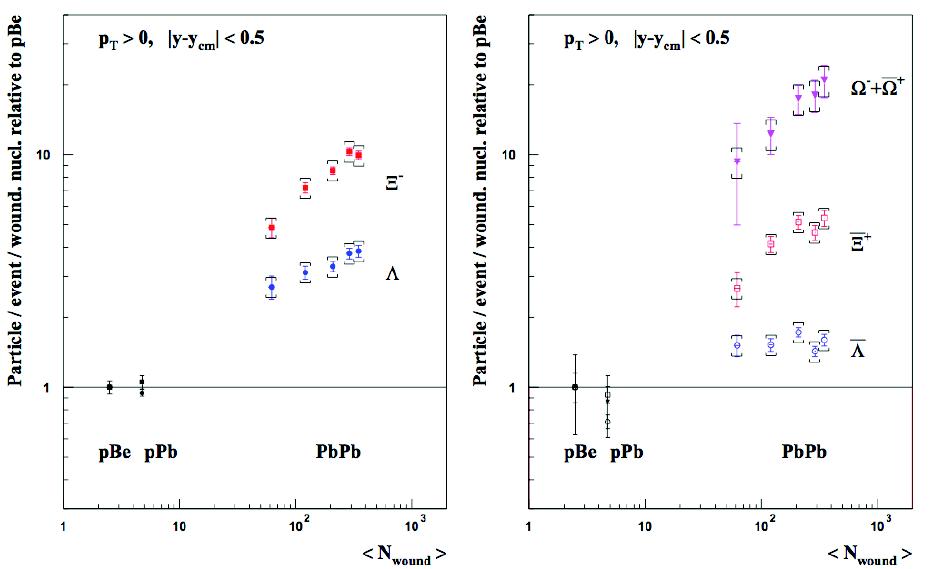
\includegraphics[width=12cm]{FigCap1/strangEnhancSPS.png}
  \caption{ Hyperon enhancement as a function of the number of the wounded nucleons measured by the NA57 experiment in Pb-Pb collisions at $\sNN = 17.2$ GeV~\cite{Sandor:2004bg}.}
  \label{fig:sEnhancSPS}
\end{figure}
For $T > T_c$, also \textit{u} and \textit{d} quark masses 
decreases to $m_q \sim 0$ MeV/$c^2$, but the 
strange quark production becomes important. In a simple hadron gas, 
even if it is possible to produce strange particles from some inelastic 
scattering such as $\pi^0+p \rightarrow K^++\Lambda$, it is less probable 
to produce multi-strange baryons, like $\Xi ^-$ and $\Omega$, as 
they are the result of more than one consecutive reactions. In presence 
of QGP, instead, it is expected an enhancement in the production of 
multi-strange baryons relative to pp reactions of about one order of magnitude.
The abundant strangeness production in QGP is due to the large gluon 
density of the system, which favours gluon-fusion processes
$gg \rightarrow s\bar{s}$. 
The Grand Canonical (GC) formulation is used whenever the conservation law of
a quantum number, for example strangeness, can be on average implemented by using
the corresponding chemical potential. This approach can be used in systems 
with a large number of produced particles. For smaller systems like pp or pA
collisions, this is no longer valid and the Canonical (C) formulation must be used
in turn. The canonical conservation of quantum numbers strictly reduces the phase
space available for particle production~\cite{Beutler:2009cc}, and this is usually referred to as canonical suppression~\cite{Tounsi:2001ck}.
This is the essence of the strangeness enhancement from pp to AA collisions.\\
In experiments the magnitude of strangeness production is usually estimated by measuring 
the enhancement factor, defined as the ratio of the yields of a given particle 
specie per participant nucleon in nucleus-nucleus collisions over the same 
ratio measured in smaller system (pp or pA). The first evidence of 
strangeness enhancement was measured by the NA57 and WA97 
collaborations~\cite{Sandor:2004bg} in fixed-target Pb-Pb collisions at 
$\sqrt{s_{NN}}$= 17.2 GeV. The enhancement factor measured by NA57 
is shown in Fig.~\ref{fig:sEnhancSPS} for $\Lambda$, $\Xi^-$ (left) and 
their anti-particles (right) in p-Pb, p-Be and Pb-Pb collisions as a function 
of the number of participating nucleons. It is observed a hierarchy for these 
enhancement factors in Pb-Pb collisions, depending on the strangeness
 content of the particles and also on the collision centrality. In p-Be and in 
 p-p there is no evidence of strangeness enhancement. 

\subsection{Collective flow and kinetic freeze-out}
\label{sec:FlowIntro}
The ``flow'' of particles produced in the interaction is a collective phenomenon, which is observed as a collective 
motion pattern superimposed to the chaotic thermal motion of the 
particles inside the fireball. Its origin is related to the large pressure gradients 
generated when compressing and heating nuclear matter. It is possible 
to distinguish between different types of flow. In the following, 
the radial and the anisotropic flow in the transverse plane are discussed. 

\subsubsection{Radial flow}
\label{sec:RadialFlow}
Regarding the particle production in pp collisions, 
following the approach in~\cite{Schnedermann:1993ws}, we 
can treat the invariant yield of low $\pt$ particles of a given species as radiated by a
 thermal source with temperature $T$, according to the Boltzmann distribution:
\begin{equation}
\label{eq:ThermalSource}
E\frac{{\rm d}^{3}n}{{\rm d}^3p} = \frac{{\rm d}n}{{\rm d}y \; m_{\rm T} {\rm d}m_T\;{\rm d}\varphi} = \frac{gV}{(2\pi)^3}E\;e^{-(E-\mu)/T},
\end{equation}
  where $g$ is the spin-isospin degeneracy factor for the considered particle 
  species, $\mu$ is the grand canonical potential $\mu = n\mu_{B}+ s\mu_S$, 
  originating from the quantum numbers $n$ and $s$ for baryon and 
  strangeness content, $y$ is the rapidity, $m_{\rm T}$ the transverse 
  mass and $\hbar = c = k_B = 1$. By integrating Eq.~\ref{eq:ThermalSource}
   over rapidity and $\varphi$, using the modified Bessel function $K_1$, we obtain
    the transverse mass distribution ${\rm d}n/(m_T{\rm d}m_T)$, which behaves 
    asymptotically like a decreasing exponential for transverse masses 
    larger than the source temperature: 
\begin{equation}
\label{eq:SpectraBZ}
\frac{{\rm d}N}{m_T {\rm d}m_T} = \frac{V}{2\pi^2} m_T K_1 (\frac{m_T}{T}) \xrightarrow{m_T \gg T} V^\prime \sqrt{m_T} e^{-m_T/T}.
\end{equation}
It has been experimentally verified in pp collisions the universality, at low $\pt$,
of the temperature $T$ of the exponential slope of Eq.~\ref{eq:SpectraBZ}. 
In the low-$\pt$ region ($\lesssim 1 \, \Gevc$), indeed, particles originate from soft processes
and their production is governed by a Boltzmann exponential distribution. 
This law does not anymore describe production at higher $\pt$, where hard processes
govern particle emission and the production spectra are better reproduced by power law functions.
 $T_{\rm slope}$ can be interpreted as the temperature of the particle
 emitting source. The universality of $T_{\rm slope}$ for different 
 particle species is commonly referred to as $m_{\rm T}$-scaling. When 
 moving to nucleus-nucleus collisions, a breaking of the $m_T$-scaling 
 occurs at low $\pt$ and the slopes of the spectra are observed to 
 decrease with increasing particle mass~\cite{Appelshauser:1998yb,Arnaldi:2007ru}.
  The effect is present at all centralities, but it is stronger for central
   collisions. The slope of the exponential law, at low $\pt$, can be expressed as:
\begin{equation}
\label{eq:Tslope}
T_{\rm slope} = T_{\rm fo} + \frac{1}{2}m \beta_{\rm T}^{2},
\end{equation}
where the second term accounts for the dependence on the mass 
and the velocity is related to the radial flow, i.e. the collective velocity
 arising from the expansion of the fireball. The first term still accounts
  for the Brownian motion of the particles, present in Eq.~\ref{eq:SpectraBZ}.
   This is the idea developed within the Boltzmann-Gibbs blast-wave 
   model~\cite{Schnedermann:1993ws}, where the radial expansion 
   velocity distribution $\beta_{\rm T}(r)$ in the region \mbox{$0 \leq r \leq R$} 
   is parametrized by relating it to the surface velocity $\beta_s$ via:
\begin{equation}
\label{eq:Br}
\beta_{\rm T} (r) = \beta_s \Big(\frac{r}{R}\Big )^n,
\end{equation}
where the exponent $n$ is used to tune the shape of the spectra profile.
\begin{figure}[!t]
  \centering
%   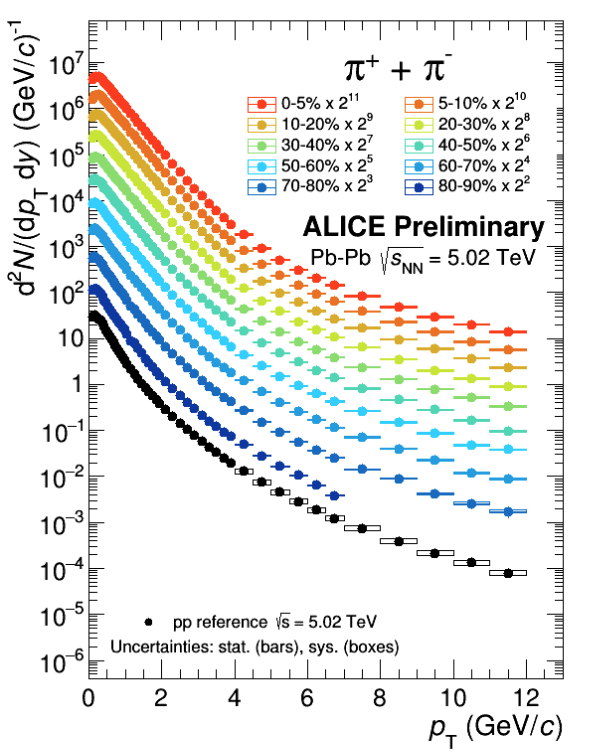
\includegraphics[height=7cm]{FigCap1/PionsPbPb5TeV.png}
   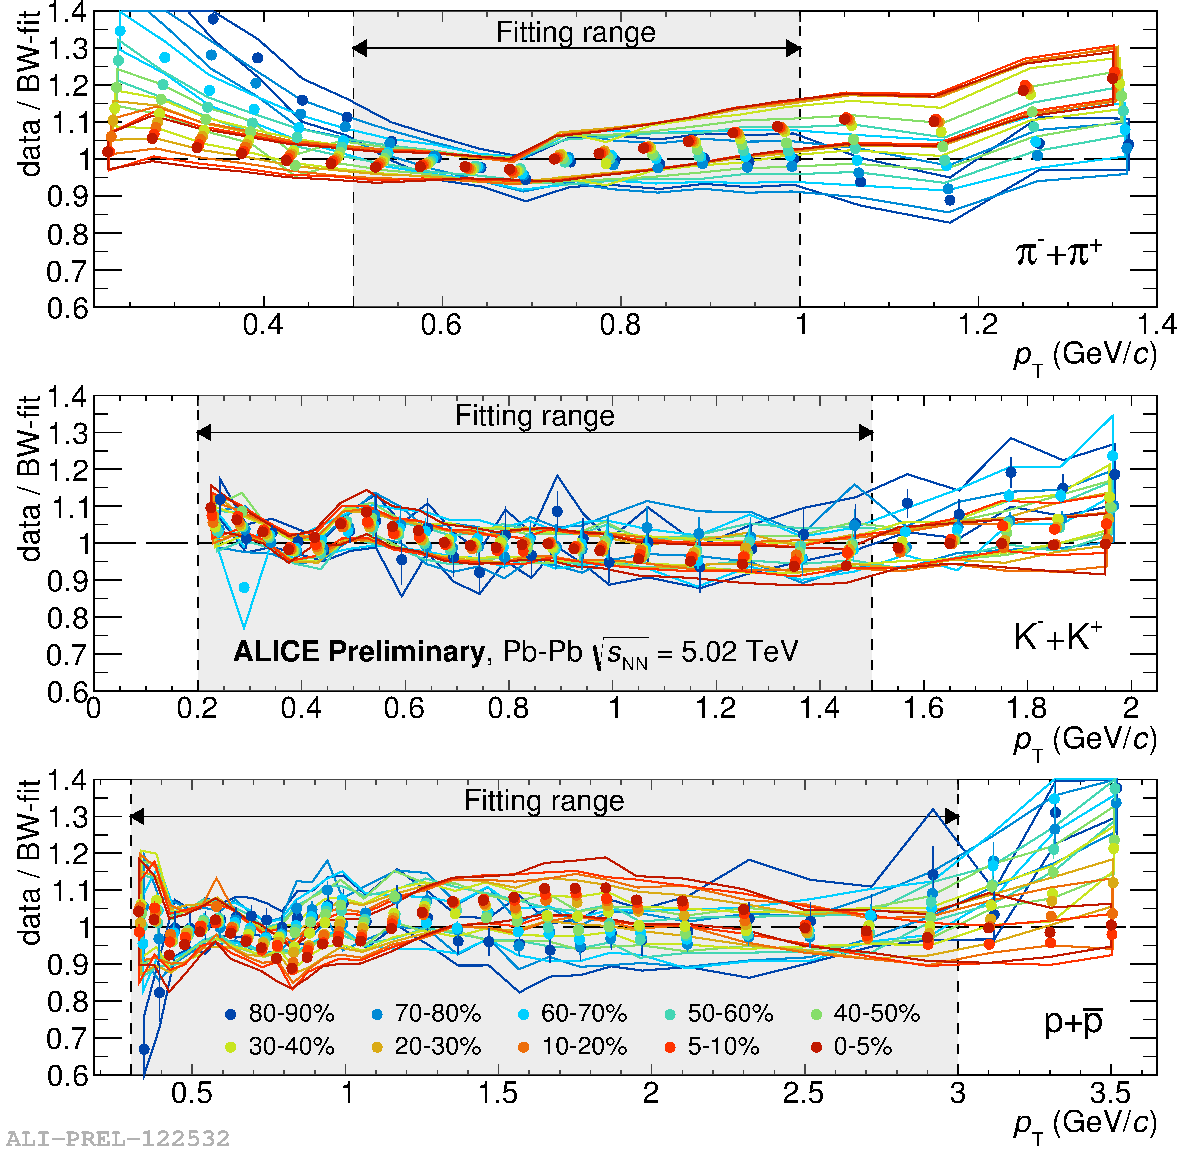
\includegraphics[height=8cm]{FigCap1/BW_5TeV.pdf}
 \caption{Ratio data to blast-wave fit for $\pi, k, p$ spectra as a function of $\pt$ in different centrality classes in Pb-Pb collisions at $\sNN = $ 5.02 TeV~\cite{Jacazio:2017dvy}, measured by ALICE.}
  \label{fig:BWfit}
\end{figure}
\begin{figure}[!t]
  \centering
  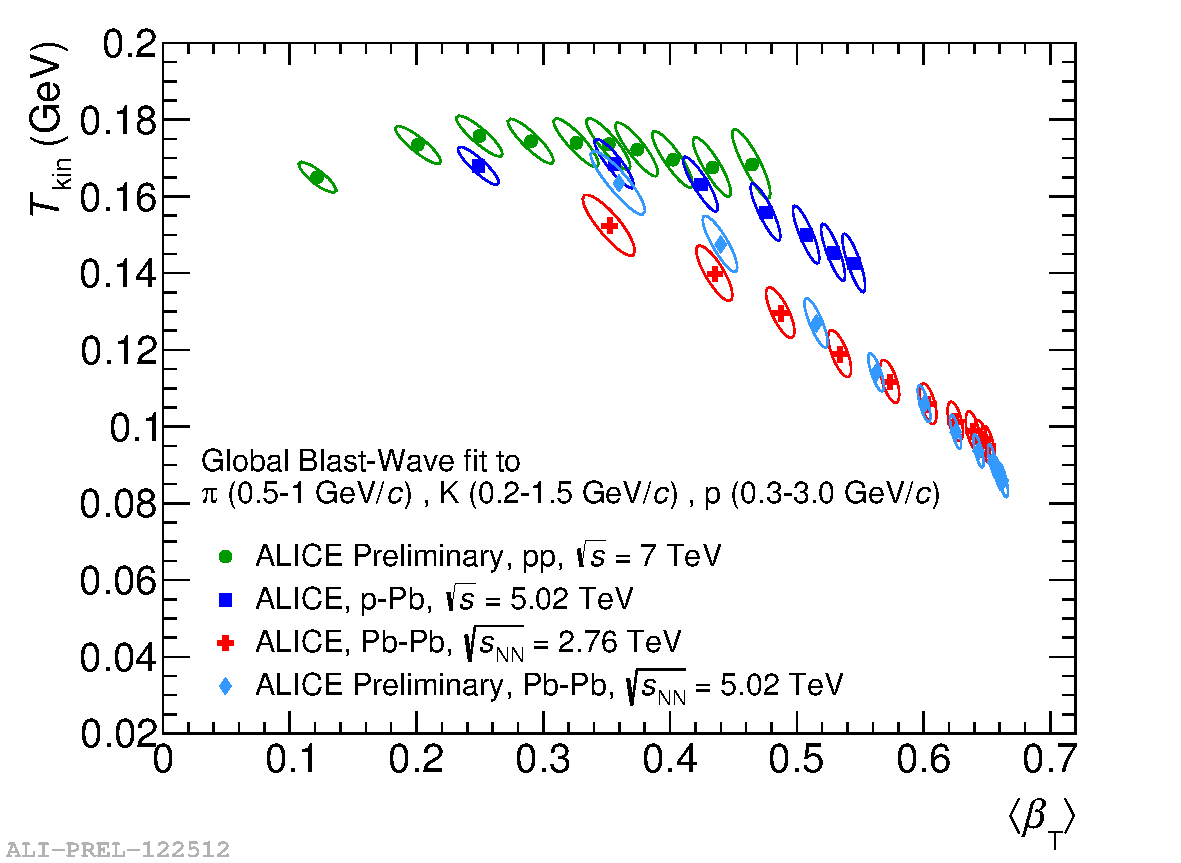
\includegraphics[height=6cm]{FigCap1/BWfit_BetaTplot.pdf}
 \caption{$T_{kin}$ vs $\langle \beta_T \rangle$ from blast-wave fits for different colliding systems and energies~\cite{Jacazio:2017dvy}.}
  \label{fig:BetaTplot}
\end{figure}

The observed particle spectrum results from the sum 
of the spectra of individual thermal sources each boosted with the 
boost angle $\rho = \tanh^{-1}(\beta_{\rm T})$:
\begin{equation}
\label{eq:BlastWave}
\frac{{\rm d}N}{\pt {\rm d}\pt {\rm d}\phi {\rm d}y}\propto \int_{0}^{R} r {\rm d}r\;  m_{\rm T}\;  K_{1} \; (\frac{m_{\rm T} \cosh(\rho(r))}{T_{\rm fo}})\;  I_{0}\; (\frac{\pt \sinh(\rho(r))}{T_{\rm fo}}).
\end{equation}
It is a three parameter ($T_{\rm fo}, \beta_s, n$) simplified hydrodynamical model.
The blast-wave fit to the measured spectra allows
  an estimate of the kinetic freeze-out temperature $T_{\rm fo}$ and 
  radial velocity $\beta_{\rm T}$. An example of data to blast-wave fit for the 
  measured spectra of pions, kaons and protons in Pb-Pb collisions at $\sNN = $ 5.02 TeV 
   by ALICE is shown in Fig.~\ref{fig:BWfit}, as a function of $\pt$ (different centrality classes 
   are in different colours).
  
Fig.~\ref{fig:BetaTplot} shows the ALICE results 
for the blast-wave parameters for different colliding systems and energies. Blast-wave parameters
  in Pb-Pb collisions at $\sNN = 5.02$ TeV follow the trends with collision centrality observed at
   lower energy ($\sNN = 2.76$ TeV). The largest expansion velocity 
   is found for central Pb-Pb collisions, as well as the lowest temperature
    for the kinetic freeze-out.\\

\subsubsection{Anisotropic flow}
\label{sec:AnisotropicFlow}
The anisotropic flow is characteristic of non-central collisions, where the 
finite impact parameter creates a fireball with a geometrical anisotropy. 
Due to particle re-scatterings during the system evolution, the initial spatial 
anisotropy is transferred to a final state momentum-space anisotropy. Absence of
 re-scatterings during the system evolution or any delays in time of such 
 interactions would lead to null momentum anisotropy in the final state or
  to a decrease in the elliptic flow signal. Hence, the characterisation of 
  anisotropic flow is important as it is sensitive to particle interactions occurring very 
  early in the system evolution. Information of medium properties, such as Equation of 
  State, sound velocity or shear viscosity can be extracted by a comparison 
  of the measured anisotropic flow and hydrodynamic model calculations.
\begin{figure}[!ht]
  \centering
  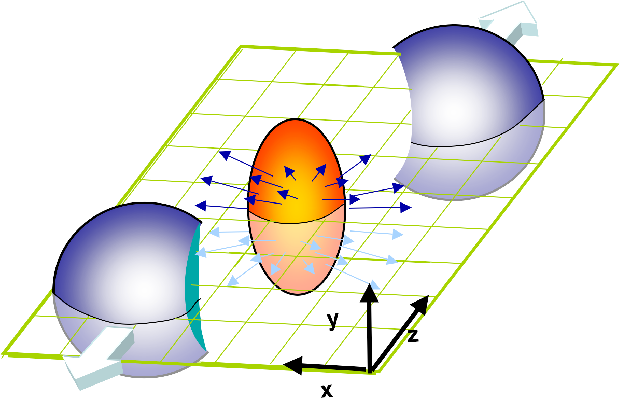
\includegraphics[width=8cm]{FigCap1/elliptic_flow_3D_medium.png}
  \caption{Picture of a semi-peripheral collision and the pressure gradients arising from a geometrical anisotropy.}
  \label{fig:elliptic_flow_3D_medium}
\end{figure}
In non-central heavy-ion collisions, an almond-shaped interaction 
volume is created in the overlap region (see Fig.~\ref{fig:elliptic_flow_3D_medium}).
The reaction plane is defined by the collision impact parameter and the 
beam line ($xz$ plane in Fig.~\ref{fig:elliptic_flow_3D_medium}). 
A pressure gradient larger in the
 reaction plane than in the plane perpendicular to it is expected. This generates an
  anisotropy in azimuthal distributions of the particle momenta with 
  respect to the reaction plane, which can be detected in the measured
   particle azimuthal distributions. This distribution can be parametrized 
   through a Fourier series decomposition:
\begin{equation}
\label{eq:FourierAzimuthExpansion}
E \frac{{\rm d}^3N}{{\rm d}^3p} = \frac{1}{2\pi} \frac{{\rm d}^2N}{\pt {\rm d}\pt {\rm d}y} (1 + \sum_{n=1}^\infty 2v_n {\rm cos} (n(\varphi - \Psi_r))),
\end{equation}
where $\varphi$ is the azimuthal direction of the emitted particle and 
$\Psi_r$ denotes the (true) reaction plane angle.
In the formula, {\it v$_n$} are the Fourier coefficients, and they can be 
evaluated as $v_n = \langle cos(n(\varphi - \Psi_r)) \rangle$, where 
$\langle \rangle$ indicates an average over all particles in all events with
 their azimuthal angle $\varphi$ in a given rapidity and $\pt$ momentum at
  a fixed centrality. The sine terms vanish due to the reflection simmetry 
  with respect to the reaction plane. {\it Direct} and {\it elliptic flow} 
  are common terms for the first and the
second order Fourier coefficients respectively in the particle azimuthal 
distribution in Eq.~\ref{eq:FourierAzimuthExpansion}, but coefficients 
up to at least 6$^{\rm th}$ order were measured at the LHC~\cite{ATLAS:2012at}.
With the large amount of data provided by the LHC, in fact, we have the possibility
to study not only the average anisotropies but also the initial space geometries 
fluctuations~\cite{Aad:2013xma,Schukraft:2012ah}, to which first-order and higher-order Fourier 
coefficients were indeed found to be sensitive. 
The positions of the nucleons in the overlap region of the colliding nuclei 
can fluctuate to create matter distributions asymmetries~\cite{Teaney:2010vd,Alver:2010dn,Alver:2010gr}, which are converted into 
non-zero first-order and higher-order harmonic coefficients. 
Fig.~\ref{fig:vnHydro} shows
   comparison to viscous hydrodynamics calculations~\cite{Gale:2012rq} of the 
   Fourier coefficients $v_n$ up to 5$^{\rm th}$ order measured by ATLAS~\cite{ATLAS:2012at}
    (left panel) in Pb-Pb collisions at $\sNN = 2.76$ TeV and 
    PHENIX~\cite{Adare:2011tg} and STAR~\cite{Pandit:2012mq} 
    (right panel) in Au-Au collisions at $\sNN = 200 $ GeV. A value
     of the shear viscosity $\eta/s$ of the medium equal to 0.12 allows a good parametrisation 
     of hydro calculations for Au-Au collisions at top of RICH energy, while a value of 0.2 is found
      for Pb-Pb collisions at the LHC at $\sNN = 2.76$ TeV.
      This reveals a dependence of the shear viscosity on the temperature of the system.
\begin{figure}[!ht]
  \centering
  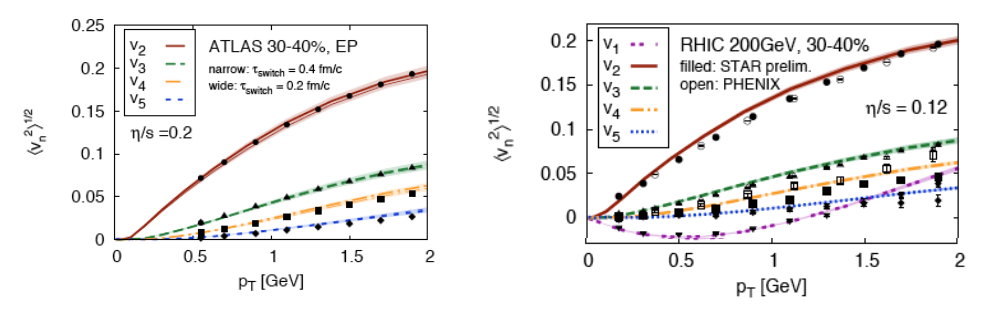
\includegraphics[width=15cm]{FigCap1/RICH_ATLAS_vn.png}
  \caption{Fourier components of anisotropic transverse flow, $v_n(\pt)$, for Pb-Pb collisions at the LHC (left panel) and for Au-Au collisions at RICH (right panel), in comparison with viscous hydrodynamics calculations~\cite{Gale:2012rq}.}
  \label{fig:vnHydro}
\end{figure}
\begin{figure}[!ht]
  \centering
  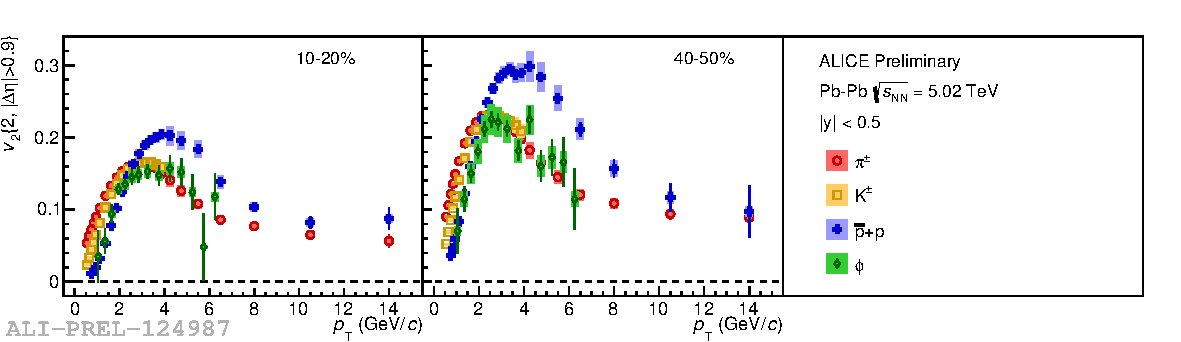
\includegraphics[width=15cm]{FigCap1/v2IdentifiedParticles.pdf}
  \caption{Elliptic flow coefficient $v_2$ of $\pi^{\pm}, K^{\pm}, p(\bar{p})$ and $\Phi$ meson for 10-20\% (left) and 40-50\% (right)
collision centrality as function of $\pt$~\cite{Bertens:2017krr}. Statistical uncertainties are shown as bars and systematic uncertainties as boxes.}
  \label{fig:v2IdentifiedParticles}
\end{figure}
Fig.~\ref{fig:v2IdentifiedParticles} shows the $\pt$-differential 
$v_2$ of $\pi^{\pm}, K^{\pm}, p(\bar{p})$ and $\Phi$ mesons for 10-20\% (left)
and 40-50\% (right) collision centrality, measured by 
ALICE in Pb-Pb collisions at $\sNN = 5.02$ TeV~\cite{Bertens:2017krr}.
For $\pt < 2$ $\Gevc$, one can notice that the $v_2$ of the different species
 follows a mass ordering, which is expected for a hydrodynamically expanding 
 source and is indicative of collective radial flow.
For 3 $< \pt < 8$ $\Gevc$, particles are grouped according to the number of their valence
 quarks, rather than their mass, which supports the
hypothesis of particle production via quark coalescence~\cite{Molnar:2003ff}. 
The non-zero $v_2$ at high $\pt$ is attributed to path-length dependent 
in-medium energy loss which is discussed in the next section~\cite{Gyulassy:2000gk}. The $\phi$ meson, 
with its mass close to proton mass, is a very good probe of quark scaling and 
mass ordering. Indeed, the $\phi$-meson $v_2$ follows proton $v_2$ at low 
$\pt$, but pion $v_2$ at intermediate $\pt$. \\

\label{sec:ChiralSymm}
\begin{figure}[!ht]
  \centering
  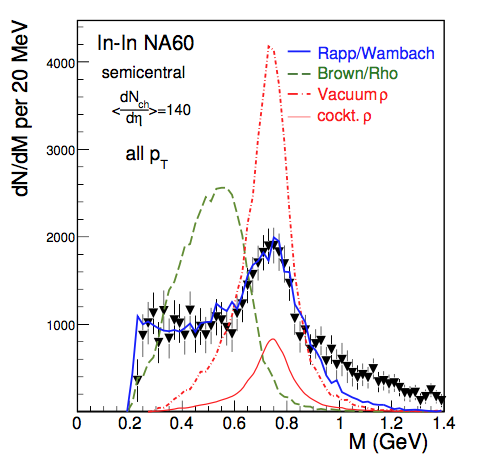
\includegraphics[width=7.2cm]{FigCap1/rhoMelting.png}
  \caption{Di-muon pair invariant mass distribution after 
background subtraction to the $\rho$ meson peak, for In-In collisions at d$N_{ch}$/d$\eta$ = 140, compared to model predictions~\cite{Rapp:2012zq}.}
  \label{fig:rhoMelting}
\end{figure}
\subsection{Chiral symmetry restoration}
If, on one side, chiral symmetry restoration should play a role in the 
observed strangeness enhancement (see Sec.~\ref{subsec:StrangEnhancSPS}),
on the other hand, signatures of this effect could also be found in the line shape of the
invariant mass distribution of thermal low-mass ($< 1$ GeV/$c^2$) dileptons.
Their production is in fact largely carried by light 
vector mesons $\rho, \omega$ and $\phi$. For this reason their are ideal to investigate
changes in the vector-meson mass distributions as the critical temperature for chiral
restoration is approached and surpassed. Changes both in width and in mass of
the mesons were originally advocated as signatures of the chiral transition~\cite{Pisarski:1981mq}. 
Among light vector mesons, the $\rho$ meson was used from the very beginning as the test particle for in-medium 
modifications, due to the abundant production
of $\pi^+ \pi^- \rightarrow \rho$ and subsequent decay $\rho \rightarrow \mu^+ \mu^- $ 
with a lifetime of 1.3 fm/c, shorter than the time between hadronization and the thermal freeze-out. 
Fig.~\ref{fig:rhoMelting}  shows NA60 measurement of the 
low-mass di-muon pair invariant mass distribution after 
subtracting the background to the $\rho$ meson peak, 
measured in In-In collisions at top SPS energy~\cite{Damjanovic:2005ni}. The $\rho$ meson is
clearly broadened in the medium as compared to the vacuum case, 
while no sign of mass shift is observed. The measurement
was found to be in good agreement with models describing an in-medium broadening 
scenario (Rapp/Wambach~\cite{Rapp:2012zq}).

\subsection{Jet quenching}
\label{sec:JetQuenching}
Partons produced in the hard scattering processes occurring in the early stages of the 
collisions fragment into collimated cascades of hadrons, called jets. 
In heavy-ion collisions partons propagate inside the hot and dense QGP,
 and lose energy because of interactions with the colored medium 
 (jet quenching), primarily via gluon radiation and, to smaller extent, 
 elastic scattering~\cite{Qin:2015srf}. The energy loss ($\Delta E$) carries 
 important information about transport coefficients 
 of the QGP (different for radiative or collisional processes), because it
  is expected to be dependent on the opacity 
 (associated to the medium density and the interaction strength) 
 and on the path length $L$ traversed by the parton inside the medium.
  Different models predict linear and quadratic dependences on $L$ 
  of the energy loss for elastic~\cite{Thoma:1990fm} and radiative~\cite{Baier:1996sk} 
  collisions respectively (a cubic dependence is predicted within the 
  AdS/CFT framework). Furthermore, $\Delta E$ also depends on the 
  color charge (different for quarks and gluons) and on the quark mass, 
  as it will be discussed in Sec.~\ref{sec:HFEnLossinAA} focusing in more detail on the heavy flavour quarks.\\

\begin{figure}[!ht]
  \centering
  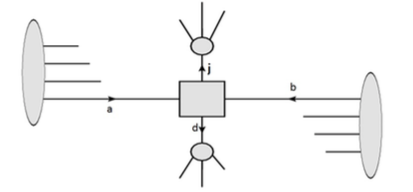
\includegraphics[width=10cm]{FigCap1/Scattering.png}
  \caption{Schematic illustration of high $\pt$ hadron production in high-energy nuclear collisions. }
  \label{fig:Scattering}
\end{figure}

In perturbative QCD, the production cross-section for a hadron $h$ 
from a process involving high-momentum transfer can be described 
using a factorisation approach as a convolution of the incoming parton distribution functions (PDFs) 
inside the nucleons, the hard partonic scattering cross-section and 
the final state fragmentation function (FFs):
\begin{equation}
\label{eq:QCDhardProduction}
\begin{split}
{\rm d}\sigma_{pp\rightarrow hX} \approx \sum_{abjd}\int {\rm d}x_a \int {\rm d}x_b \int {\rm d}z_j f_{a/p} (x_a, \mu_f) \; \otimes \;f_{b/p} (x_b, \mu_f) \;\otimes \\
{\rm d}\sigma_{ab \rightarrow jd} (\mu_f,\mu_F,\mu_R) \otimes D_{j\rightarrow h} (z_j,\mu_F), 
\end{split}
\end{equation}
where $x_a$, $x_b$ are the initial nucleon momentum fractions carried by the
 interacting partons, $z_j = p_h/p_j$ is the parton momentum 
 fraction carried by the final observed hadron. Then, $f_{a/p} (x_a, \mu_f)$
  and $f_{b/p} (x_b, \mu_f) $ are the parton distribution functions, 
  ${\rm d}\sigma_{ab \rightarrow jd} (\mu_f,\mu_F,\mu_R) $ is the differential 
  cross-section for parton scattering process and $D_{j\rightarrow h} (z_j,\mu_F)$
   is the fragmentation function for parton $j$ to hadron $h$, which represents
    the probability for a parton to hadronize into a hadron carrying a fraction $z$ 
    of the parton momentum. Finally, $\mu_f$ and $\mu_F$ are the factorisation 
    scales and $\mu_R$ is the renormalisation scale. The PDFs are measured 
    at a given $Q^2$ in experiments of deep inelastic scattering and evolved
     to different energy scales using DGLAP equations~\cite{Altarelli:1977zs}.
      Fragmentation functions cannot be calculated with pQCD and are usually 
      tuned on measurement in $e^+e^-$ collisions.\\


The inelastic differential cross-section for nucleus-nucleus interaction, derived from Eq~\ref{eq:sigmaABGlauber} 
under the assumption of the optical Glauber model, is:
\begin{equation}
\label{eq:sigmaABGlauberDiff}
\frac{{\rm d}\sigma^{\rm inel}_{\rm AB}}{{\rm d}\vec{b}} = 1 - [1-  T_{\rm AB}(\vec{b})\sigma^{\rm inel}_{\rm NN}]^{\rm AB},
\end{equation}
where $\sigma^{\rm inel}_{\rm NN}$ is the nucleon-nucleon inelastic interaction cross-section
and $T_{\rm AB}$ is the nuclear overlap function of the two nuclei.
For hard processes, for which the cross section is small, Eq.~\ref{eq:sigmaABGlauberDiff} can be approximated as:
\begin{equation}
\label{eq:xsecHardProcesses}
\frac{{\rm d}\sigma^{\rm hard}_{\rm AB}}{{\rm d}\vec{b}} \simeq 1 - [1- {\rm AB}\, T_{\rm AB}(\vec{b})\sigma^{\rm hard}_{\rm NN}] =  {\rm AB} \,T_{\rm AB}(\vec{b})\sigma^{\rm hard}_{\rm NN} \propto \langle N_{\rm coll} \rangle \sigma^{\rm hard}_{\rm NN},
\end{equation}
where $N_{\rm coll}$ is the number of nucleon-nucleon collisions occurring
in the nucleus-nucleus interactions. 
As a consequence, in case of particles produced in hard processes, the 
Glauber Model predicts that the production yield in heavy-ion collisions is governed by the $N_{\rm coll}$ 
scaling of the yield in pp collisions.
One of the experimental observables used for the study of energy loss
 inside the QGP is the nuclear modification factor, defined as the ratio 
 between the production of particles in nucleus-nucleus collisions and 
 the one expected according to the binary scaling in nucleon-nucleon collisions:
\begin{equation}
\label{eq:Raa}
\Raa (\pt, y) = \frac{1}{N_{\rm coll}}\frac{{\rm d}^2N_{\rm AA}/\pt {\rm d}y}{{\rm d}^2N_{\rm pp}/\pt {\rm d}y}.
\end{equation}
$\Raa$ is expected to be compatible 
with unity if no medium effects are present. A measurement significantly 
different from the unity implies modifications of the transverse momentum 
distributions of the produced hadrons, that can be related to in-medium 
energy loss effects of quarks at high $\pt$. Other effects must be considered 
when studying the energy loss of partons inside the QGP, based on
measurements of modification of momentum (energy) distribution of hadrons (jets)
in A-A collisions relative to pp interactions. The first is that the PDFs of 
bounded nucleons are different from those of the free nucleons. In addition, 
other cold nuclear matter (CNM) effects could affect the measured distributions,
such as $k_{\rm T}$ broadening due to multiple scattering of the
parton in the nucleus, energy loss in CNM ... These effects 
will be discussed in Sec.~\ref{sec:CNM}.
Finally, the parton travelling across the QGP experiences energy loss (hot nuclear matter effects) 
  before fragmenting in the final state. Thus taking into account both cold and hot nuclear matter effects, 
Eq.~\ref{eq:QCDhardProduction} becomes:
\begin{equation}
\label{eq:QCDwNuclEffects}
{\rm d}\sigma_{AB\rightarrow hX} \approx \sum_{abjj\prime d} f_{a/A} (x_a) \; \otimes \;f_{b/B} (x_b) \;\otimes {\rm d}\sigma_{ab\rightarrow jd} \otimes P_{j\rightarrow j\prime} \otimes D_{h/j\prime}(z_{j\prime}), 
\end{equation}
where the additional piece $P_{j\rightarrow j\prime}$ describes the 
effects of the hard parton $j$ interacting with the colored medium 
before fragmenting into hadrons. \\

It is necessary to disentangle different contributions from cold and hot nuclear matter 
effects to have access to the medium transport properties via
 measurements of the $\Raa$. Some of the measurements of $\Raa$
  of high-$\pt$ hadrons and jets at the LHC are presented below.

\subsubsection{High-$\pt$ hadrons}
\label{sec:HighPtPartons}
Measurements of the nuclear modification factors in central heavy-ion 
collisions at four different centre-of-mass energies, for neutral pions 
($\pi^0$) (SPS~\cite{Aggarwal:2001gn,dEnterria:2004cly,Alt:2007cd},
 RHIC~\cite{Adare:2012wg}),
 charged hadrons ($h^{\pm}$) (RHIC~\cite{Adams:2003kv}), and
  charged particles (LHC~\cite{Abelev:2012hxa,Aad:2015wga,CMS:2012aa}),
   compared to predictions of two models from~\cite{Chien:2015vja,Xu:2015bbz}
    are presented in Fig.~\ref{fig:CMSRaa}. The LHC measurements at
     $\sNN = 2.76$ and 5.02 TeV show stronger suppression than SPS 
     and RHIC measurements at intermediate $\pt$. CMS extended the measurement of the 
     $\Raa$ up to 300 $\Gevc$, and the suppression in the high-$\pt$ 
     region is found to be smaller with increasing $\pt$, demonstrating 
     that even very energetic partons suffer energy loss in the medium.
      ALICE complements the picture down to $\pt = 0 \; \Gevc$, 
      showing a perfect agreement with CMS and ATLAS in the intermediate-$\pt$ region.
\begin{figure}[!ht]
  \centering
  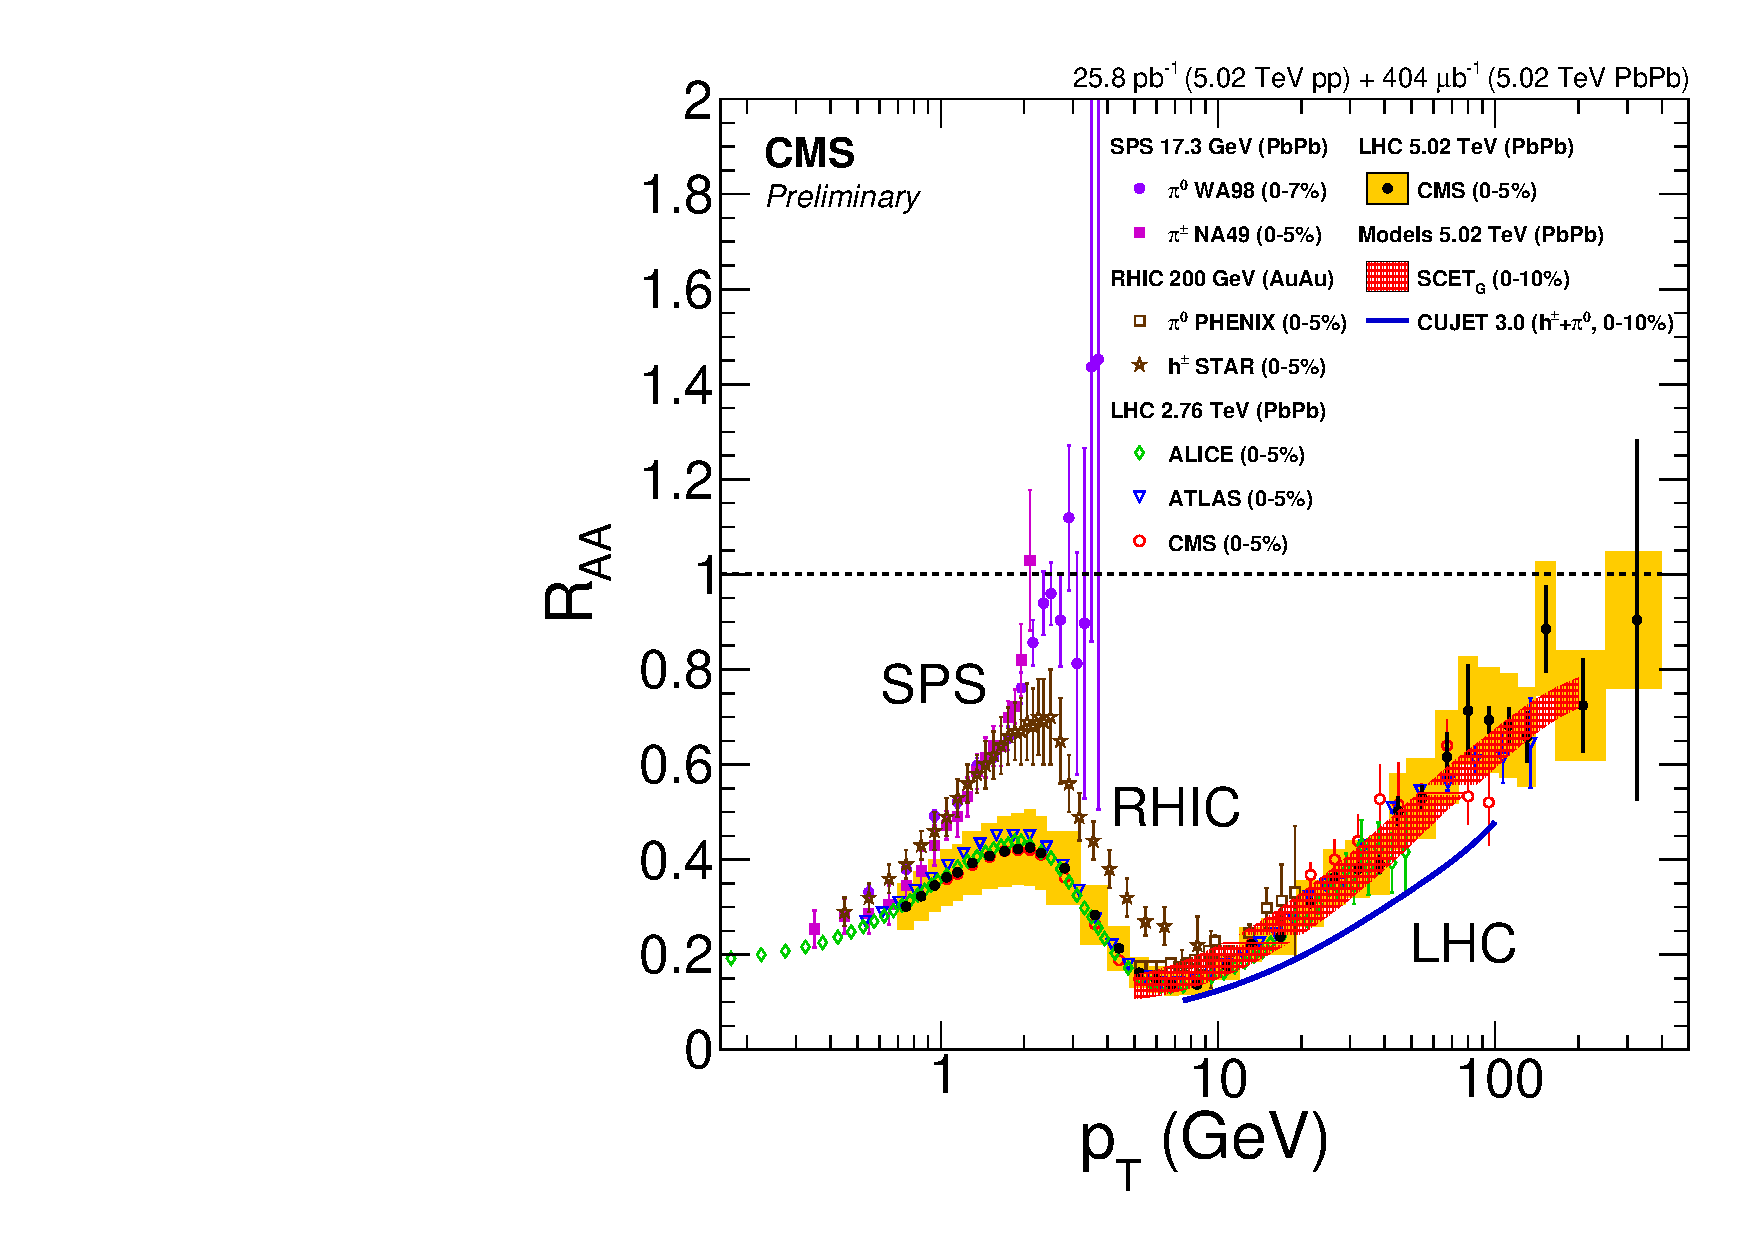
\includegraphics[width=8cm]{FigCap1/CMSRaa.pdf}
  \caption{Measurements of the nuclear modification factors in central heavy-ion collisions at four different center-of-mass energies at SPS~\cite{Aggarwal:2001gn,dEnterria:2004cly,Alt:2007cd}, RHIC~\cite{Adare:2012wg,Adams:2003kv}, and LHC~\cite{Abelev:2012hxa,Aad:2015wga,CMS:2012aa}, compared to predictions of two models from~\cite{Chien:2015vja,Xu:2015bbz}.}
  \label{fig:CMSRaa}
\end{figure}
ALICE also measured the nuclear modification factor of identified 
particle species, that can further constrain the models. In Fig.~\ref{fig:PiKPRaa5TeV}
 the $\Raa$ of pions, kaons and protons measured in Pb-Pb collisions 
 at $\sNN = 5.02$ TeV is shown, for different centrality classes. First, it 
 has to be noticed that the suppression has a clear dependence on the 
 collision centrality. It becomes stronger in more central events, 
 where the medium is more spatially extended, hotter and denser. 
 A second observation from 
  results in Fig.~\ref{fig:PiKPRaa5TeV} is that there is a mass ordering at 
  low $\pt$ that is a direct consequence of the radial flow. In fact, in the low-$\pt$
  region, where the particle yields in A-A collisions are not governed by the $N_{\rm coll}$ scaling 
  of the yields in pp collisions, the particle spectra are harder in A-A than in pp collisions due to the radial flow, which 
 is present at all centralities, but is stronger for central collisions and
  is more pronounced for massive particles.
  At high $\pt$ instead, the suppression is similar for the three species. Different model calculations were compared to the $\Raa$ 
    measured in different centrality classes by CMS~\cite{CMS:2012aa} 
    and ALICE~\cite{Abelev:2012hxa} and allowed for an extraction of 
    the transport coefficient~\cite{Baier:1996sk} $\hat{q} \approx 1.7-1.9$ 
    GeV$^2/c$ illustrated in~\cite{Burke:2013yra,Liu:2015vna}. 
\begin{figure}[!ht]
  \centering
  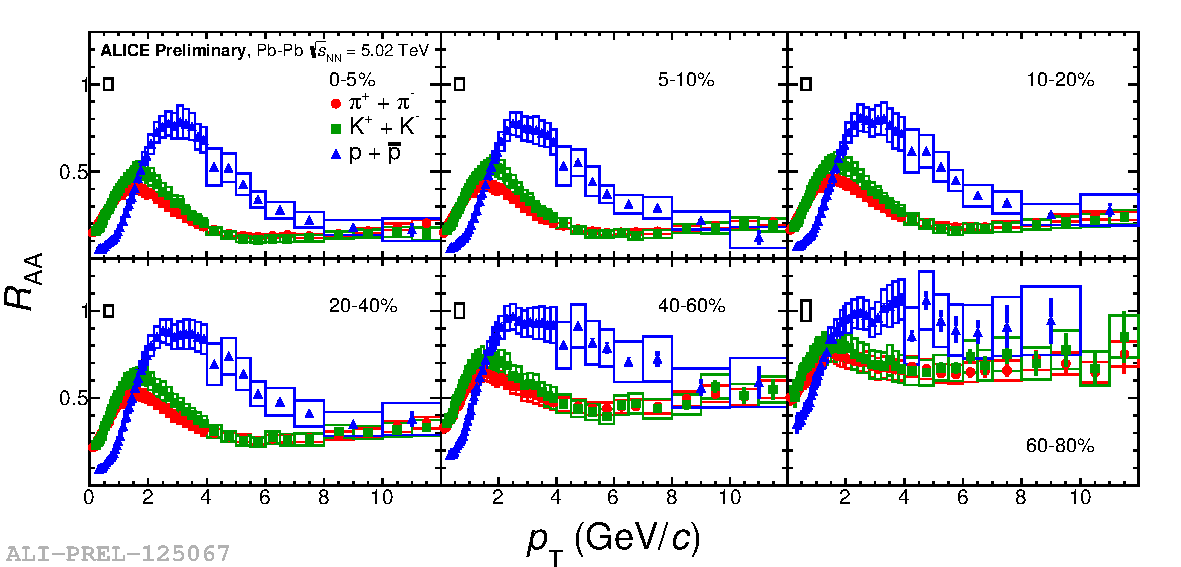
\includegraphics[width=15cm]{FigCap1/KPiPRAA5TeV.pdf}
  \caption{Nuclear modification factor of pions, kaons and protons measured by ALICE in Pb-Pb collisions at $\sNN = 5.02$ TeV in different centrality classes~\cite{Jacazio:2017dvy}.}
  \label{fig:PiKPRaa5TeV}
\end{figure}

\subsubsection{Jets}
\label{sec:Jets}
The interest in jet measurement with respect to single hadrons is that
the kinematics of the leading parton becomes accessible and we are 
less sensitive to fragmentation effects. Therefore jets are expected to put 
more stringent constraints on assumptions in models for parton energy loss. 
Experimental techniques are now able to clearly identify jets 
even in the huge background of high-energy heavy-ion collisions. 
The interaction of the high-$\pt$ partons with the color field of the medium
 induces the radiation of (mostly) soft ($\omega \ll E_{L}$, $E_L$ being the 
 energy of leading parton) and collinear ($k_{\perp} \ll \omega$, $k_{\perp}$ being
 the transverse component of the radiated gluon momentum) gluons. The 
 modeling of a jet emerging from the medium is more complex than that of
  single hadron, since not only the energy loss of the leading parton has to be 
  kept into account, but also the radiated gluons can further re-scatter in the 
  medium inside the jet cone. Thus the total energy inside the jet cone 
  of radius $R$ at the time $t_f$ is:
\begin{equation}
\label{eq:EnergyJet}
E_{jet}(t_f,R) = E_L(t_f) +E_g(t_f,R),
\end{equation}
where $E_g$ is the energy of the radiated gluons, that is defined as:
\begin{equation}
\label{eq:Eg}
E_g(t_f,R) = \int_R d\omega dk^2_\perp \omega f_g(\omega,k^2_\perp,t_f),
\end{equation}
where $f_g(\omega,k_{\perp},t)$ is the double differential distribution of 
the accompanying gluons of the leading parton. It can be obtained after solving 
the following transport equation for the distribution of radiated gluons~\cite{Qin:2015srf}:
\begin{equation}
\label{eq:RadGluonTransport}
\frac{df_g(w,k_{\perp},t)}{dt} = -\hat{e}\frac{\partial f_g}{\partial \omega} + \frac{1}{4}\hat{q}\nabla^2_{k_{\perp}}f_g + \frac{dN^{rad}_g}{d\omega dk^2_{\perp} dt}.
\end{equation}
The first and the second term in the right-hand side of Eq.~\ref{eq:RadGluonTransport} 
describe the evolution of radiated gluons which can transfer energy 
into the medium via collisional processes (controlled by coefficient 
$\hat{e}$) and accumulate transverse momentum $k_\perp$ 
(coefficient $\hat{q}$). The last term accounts for additional gluon 
radiation coming from emission of the leading parton.\\
\begin{figure}[!ht]
  \centering
  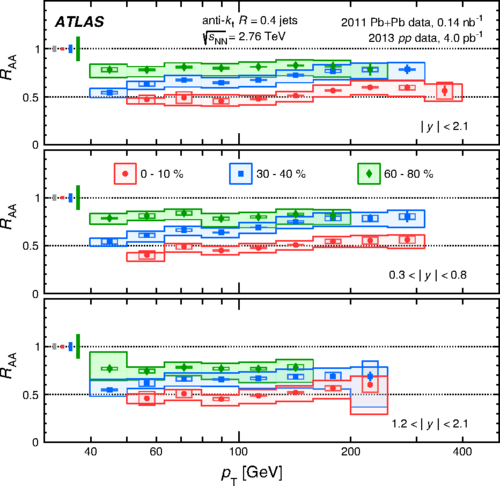
\includegraphics[width=9cm]{FigCap1/ATLASjetsRaa.png}
  \caption{Jet $\RAA$ as a function of $\pt$ in different centrality
intervals in Pb-Pb collisions at $\sNN = 2.76$ TeV~\cite{Aad:2014bxa}. Each panel shows a different range in $|y|$.}
  \label{fig:ATLASjetsRaa}
\end{figure}
\begin{figure}[!ht]
  \centering
  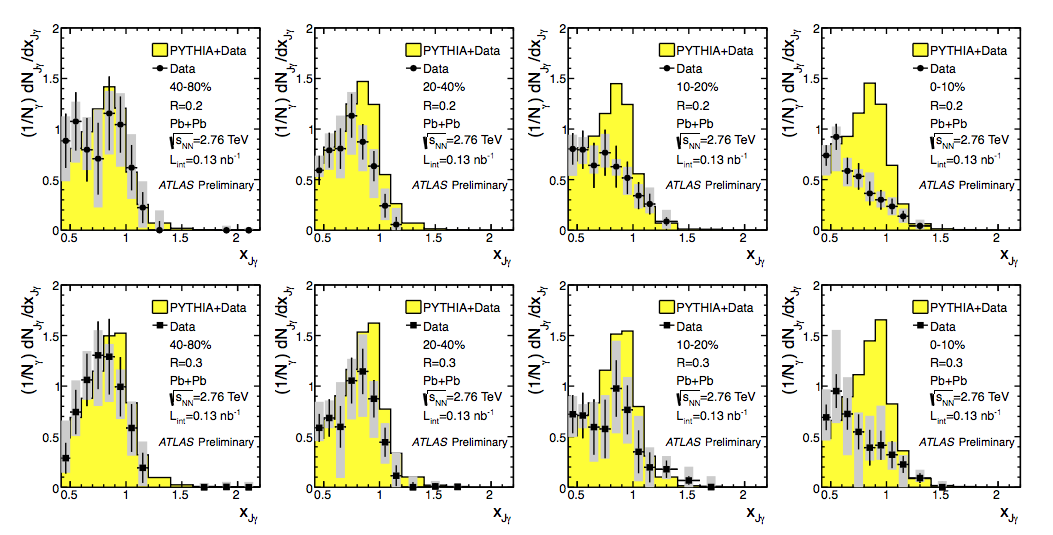
\includegraphics[width=15cm]{FigCap1/ATLASdiijetGammaZ.png}
  \caption{$\frac{1}{N}\frac{dN}{dx_J}$ distribution for reconstructed photon-jet events in Pb-Pb collisions at $\sNN = 2.76$ TeV compared to PYTHIA calculations ($x_J$ is defined in the text)~\cite{ATLAS-CONF-2012-121}. Different centrality classes are shown in each column, while the rows show results for two jet radii, R $= 0.2$ and R $=0.3$.}
  \label{fig:ATLASdijetAsymm}
\end{figure} 



Fig.~\ref{fig:ATLASjetsRaa} shows the jet $\Raa$ measured by ATLAS 
as a function of $\pt$ in different centrality classes and different 
rapidity selections for the three panels~\cite{Aad:2014bxa}. The 
suppression has a clear dependence on the event centrality, while 
is quite flat as a function of $\pt$ in the analysed range from 40 to 400 $\Gevc$. 
This result confirms the strong suppression observed for high-$\pt$ 
charged hadron yield in Pb-Pb relative to pp collisions at LHC energies and reveals that the 
medium is so opaque to quench even the most energetic jets. The 
azimuthal correlations of transverse energy of back-to-back jets 
constitute an other interesting observable to characterize the effect 
of jet-medium interaction. At LHC energies, a large number of dijet 
from back-to-back partons is observed to have an asymmetry in the energy 
of the two reconstructed jets, that can be quantified by 
$x_J = \pt^{jet1}/\pt^{jet2}$. 
In general, measurements of inclusive jets and dijet suffer from the fact that leading jets 
experience themselves some energy loss, thus the energy of the jet is not 
fully defined. Using weak bosons (Z or W) or photons, that do not interact 
with the medium, to replace one of the two jets allows us to fully calibrate the 
initial energy of the jet, as explained in~\cite{Wang:1996yh}. 
Fig.~\ref{fig:ATLASdijetAsymm} shows the $\frac{1}{N}\frac{dN}{dx_J}$ 
distribution for reconstructed photon-jet events in Pb-Pb collisions at $\sNN = 2.76$ TeV 
compared to PYTHIA calculations~\cite{ATLAS-CONF-2012-121}. 
Each column corresponds to different centrality classes, while the 
rows show results for two jet radii, R $= 0.2$ and R $=0.3$. In more 
peripheral collisions the $x_J$ distribution is peaked towards 1, thus 
meaning that higher $\pt$ dijets tend to be balanced in momentum. 
Moving towards more central events, the $x_J$ distribution appears 
flatter around $0.5 < x_J<1$, to eventually become peaked around 
$x_J \sim 0.5$ in the 10\% more central events.
This is understood in terms of different path 
lengths that the parton and the photon have to traverse in the medium. 
% \begin{figure}[!ht]
%   \centering
%   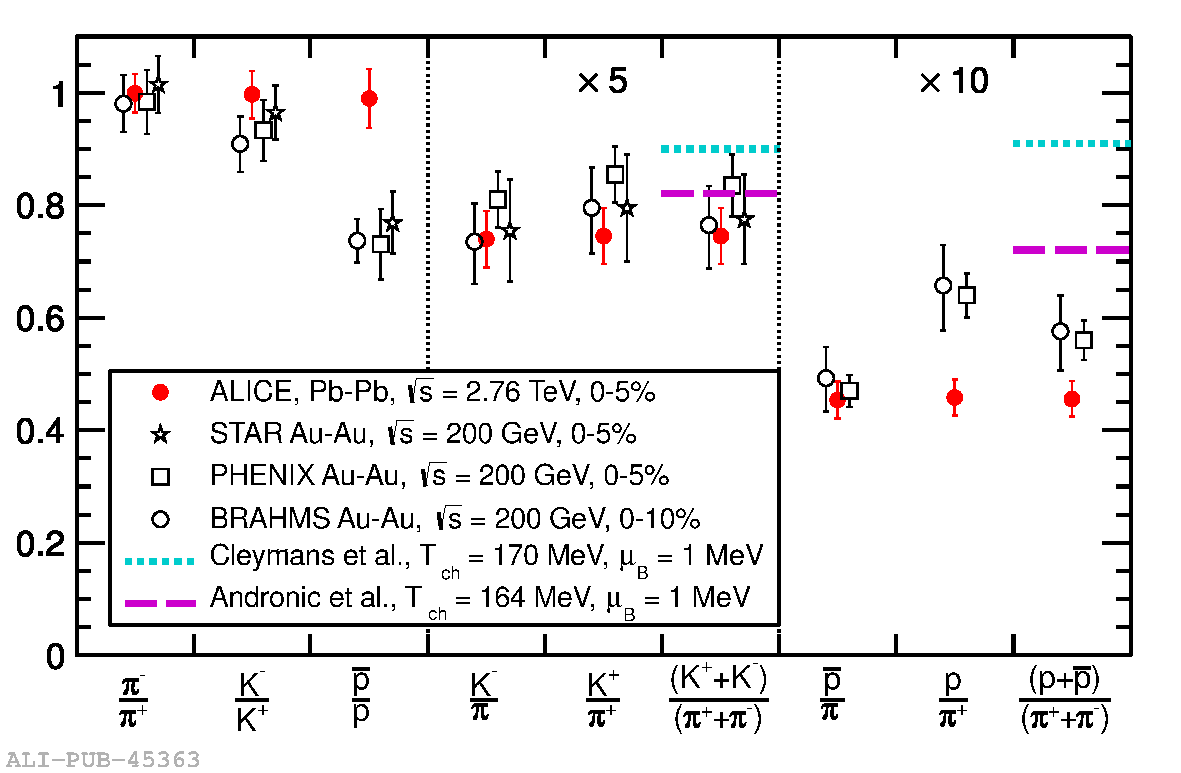
\includegraphics[width=10cm]{FigCap1/CentralPbPbRatiosThermalModels.pdf}
%   \caption{Mid-rapidity particle ratios, compared to RHIC results~\cite{Abelev:2008ab,Adler:2003cb,Arsene:2005mr} and predictions from thermal models~\cite{Andronic:2008gu,Cleymans:2006xj} for central Pb-Pb collisions at the LHC (combined statistical and systematic errors)~\cite{Abelev:2012wca}. }
%   \label{fig:CentralPbPbRatiosThermalModels}
% \end{figure}
\subsection{Quarkonium production}
\label{sec:Quarkonium}
Quarkonium, the bound state of a $c\bar{c}$ (charmonium) or $b\bar{b}$ 
(bottomonium) pair, was proposed from the very beginning as one of the 
most powerful signatures of the QGP formation.
The signature given by the J/$\psi$ vector meson production yield is of particular interest
to access information about the formation of a deconfined medium.
The J/$\psi$ mesons, and more in general the charmonium states, are formed 
by a $c\bar{c}$ quark pair, that can only be produced (due to their large mass) 
in the initial hard parton scatterings, occurring before the formation of the 
Quark-Gluon Plasma. Theoretical calculations based on lattice QCD 
predict a J/$\psi$ suppression to be induced by the screening of the color 
force in a deconfined medium, due to the presence of free 
color charges, which becomes stronger as the temperature 
increases~\cite{Abreu:2000ni,Matsui:1986dk}. 
J/$\psi$ suppression was first observed at the SPS in Pb-Pb collisions, by 
the NA38 and NA50 experiments~\cite{Abreu:2000ni}.
The ratios between the observed J/$\psi$ yield and the expected one 
based on the so-called ``ordinary nuclear absorption" measured in p-A 
collisions are shown in Fig.~\ref{fig:JPsiSuppressionNA50} 
as a function of the energy density $\epsilon$ of the medium traversed by the charmonium state. 
The results showed that for energy densities up to $\epsilon \lesssim 2$ GeV/fm$^3$, 
the yield of the J/$\psi$ meson is compatible with measurements in pp 
and p-A collisions, in which only ordinary nuclear absorption is present. In Pb-Pb 
collisions, instead, where $\epsilon$ becomes larger, there is a clear deviation from 
unity of the ratio measured/expected, which was interpreted as a first indication of 
charmonium suppression due to colour screening in the QGP~\cite{Abreu:2000ni}.
\begin{figure}[!ht]
  \centering
  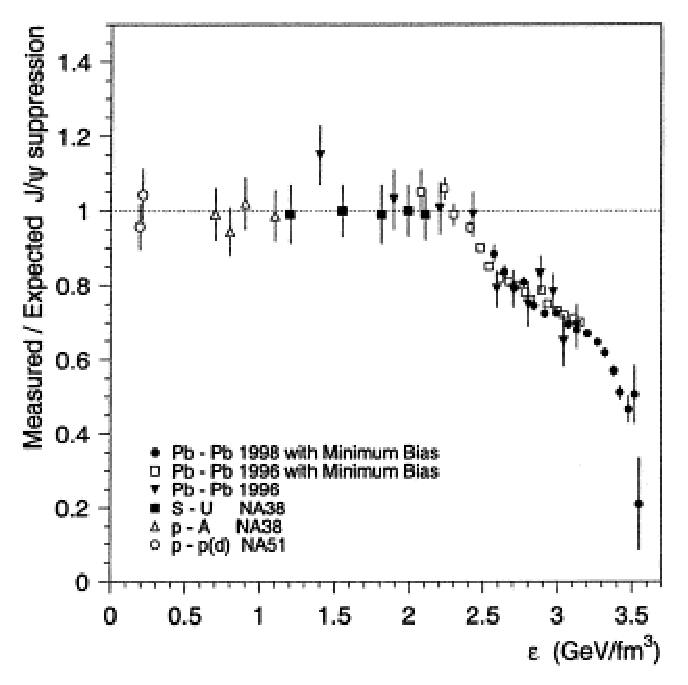
\includegraphics[width=6.6cm]{FigCap1/JPsiSuppressionNA50.eps}
  \caption{Ratio between measured J/$\psi$ production and expected one in pp, p-A and A-A collisions as function of the energy density of the medium ~\cite{Abreu:2000ni}.}
  \label{fig:JPsiSuppressionNA50}
\end{figure}
Charmonium states were also expected to melt at different temperatures of 
the plasma, accordingly to their binding energy, giving rise to a sequential melting 
scenario~\cite{Du:2015wha,Digal:2001ue}. When
data at higher collision energies became available 
at RICH~\cite{Adare:2011yf,Adare:2006ns}, results showed unexpectedly that J$/\psi$ suppression 
had the same magnitude as the one observed at the SPS~\cite{Scomparin:2007rt}.
At LHC energies, a reduced suppression as compared to lower
collision energies was observed~\cite{Abelev:2013ila}.
In Fig.~\ref{fig:RaaJPsi} the ALICE measurements 
of J$/\psi$ $\Raa$ in Pb-Pb collisions at $\sNN = 2.76$ TeV~\cite{Abelev:2013ila} 
and at $\sNN = 5.02$ TeV~\cite{Adam:2016rdg} are compared to measurements at 
RHIC~\cite{Adare:2011yf} for Au-Au collisions at $\sNN = 200$ GeV. In the left panel of Fig.~\ref{fig:RaaJPsi} 
the $\Raa$ is presented as a function of the centrality and shows smaller J$/\psi$ suppression 
at the higher energies, where the measurement is for J$/\psi$ with $\pt < 8\, \Gevc$. 
The centrality dependence is similar at the two LHC energies. 
In the right panel of the same figure, the 
dependence on $\pt$ reveals that the different suppression at different $\sNN$ is mostly
in the low-$\pt$ region.
CMS measured the J$/\psi$ $\Raa$ 
in the high $\pt$ region, up to $\pt = $ 30 $\Gevc$, confirming a stronger suppression
($\RAA \approx 0.3$ for most central events) with respect to 
low $\pt$~\cite{Khachatryan:2016ypw}. All these observations can be 
explained by a (re)generation effect of uncorrelated $c$ and $\bar{c}$ quarks, relevant at LHC energies due to the 
large production cross-section of $c\bar{c}$ quark pairs. 
Another observable sensitive to the J$/\psi$ production 
mechanism is the elliptic flow $v_2$. If we assume that the J$/\psi$ is produced by coalescence 
of charm quarks, and that the charm thermalises in the medium, the J$/\psi$ 
should inherit the flow of the quarks and show a positive $v_2$. 
Nevertheless, a non-zero $v_2$ could also be observed due to the path-length dependence of the charmonium
in-medium energy loss, thus the final $v_2$ may be an 
interplay of multiple effects. Fig.~\ref{fig:JPsi} presents recent measurements 
by ALICE of J$/\psi$ $v_2$ at forward and mid-rapidity in Pb-Pb collisions at 
$\sNN = 5.02$ TeV for semi-central events (20-40\% centrality class)~\cite{Acharya:2017tgv}, 
compared with some of the available theoretical models. At forward rapidity, 
the maximum $v_2$ is reached in $4 < \pt < 6\; \Gevc$, with a 
significance for non-zero $v_2$ larger than $6.6\sigma$. Model calculations 
including (re)combination of thermalised charm and beauty quarks as 
source of J$/\psi$ production, together with a path-length dependent in-medium 
energy loss can describe the data at low $\pt$, but fail in 
reproducing the measured shape at higher $\pt$, suggesting a missing mechanism in the 
model ({\it Du et al.} in Fig.~\ref{fig:JPsi}~\cite{Du:2015wha}). The model by 
{\it Zhou et al.}~\cite{Zhou:2014kka} includes, in addition to the cited components, 
a contribution from the modification of quarkonium production in the presence 
of a strong magnetic field in the early stage of the heavy-ion collision~\cite{Guo:2015nsa}. 
The $v_2$ resulting from the different in-plane and out-of-plane survival 
probabilities of primordial J$/\psi$ is shown as dashed red and dash-dotted 
orange lines. At LHC energies also the bottomonium states have been 
measured, opening the way to precision studies for the $\Upsilon$({\it n}S) 
family. Due to smaller production cross-section of $b$ quarks compared to $c$ quarks, 
effects of coalescence are
expected to have a smaller impact with respect to charmonium~\cite{Andronic:2015wma}. 
A sequential suppression pattern is expected also for $b\bar{b}$ states, due to 
different binding energies of the bottomonium states. CMS measured 
the $\Raa$ of $\Upsilon$(1S), $\Upsilon$(2S) and $\Upsilon$(3S) as a 
function of the centrality in Pb-Pb collisions, computed as the average number of participating
nucleons, at 
$\sNN = 2.76$ TeV~\cite{Khachatryan:2016xxp} (Fig.~\ref{fig:JPsi}, right) and at 
$\sNN = 5.02$ TeV~	\cite{Sirunyan:2017lzi}. The $\RAA$ in the right panel of Fig.~\ref{fig:JPsi} shows a 
suppression for the $\Upsilon$(2S) state, that is larger with 
respect to the $\Upsilon$(1S) state at all centralities, while for 
the $\Upsilon$(3S) only an upper limit could be determined.
The measured suppression of the three $\Upsilon$ states is compatible 
with theoretical models of a sequential melting of quarkonium states in a 
hot medium~\cite{Khachatryan:2016xxp}.
%~\cite{Sirunyan:2016znt}
\begin{figure}[!ht]
  \centering
  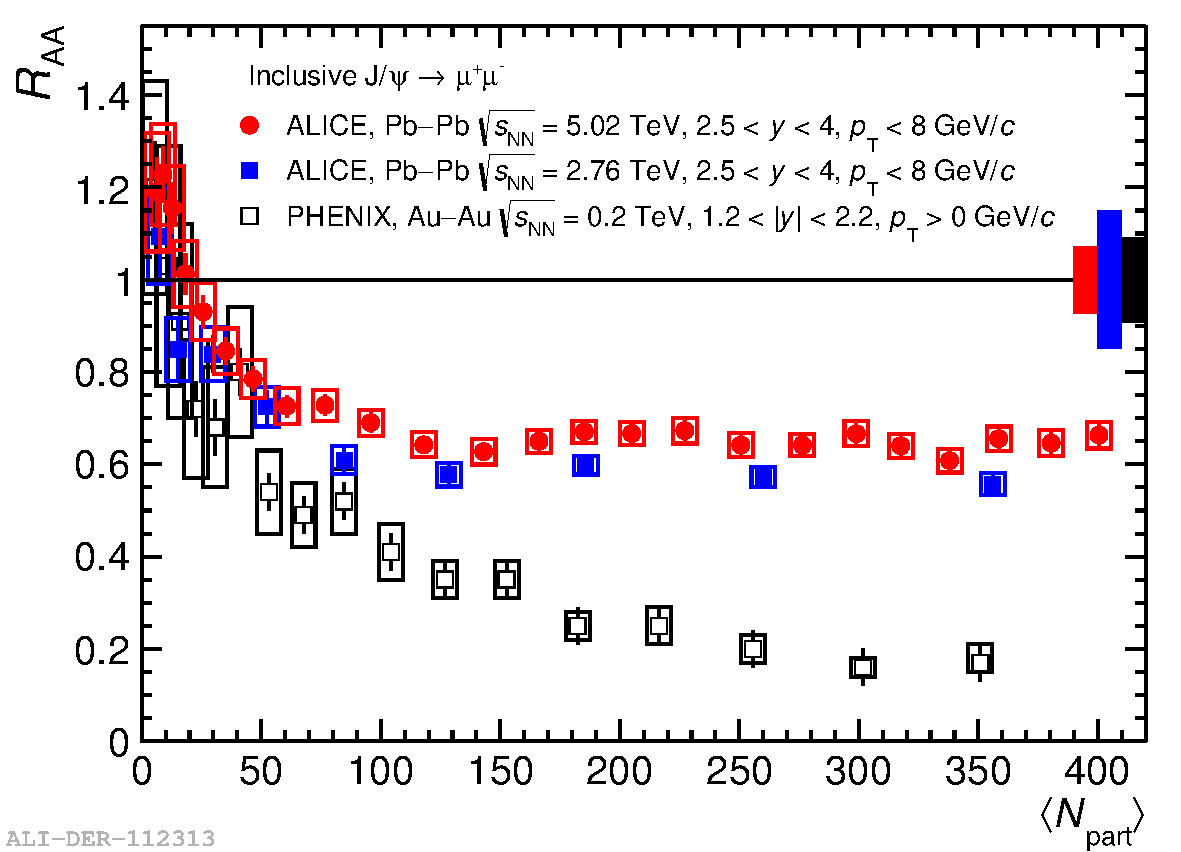
\includegraphics[width=7cm]{FigCap1/RaaJPsiAlicePhenix.pdf}
  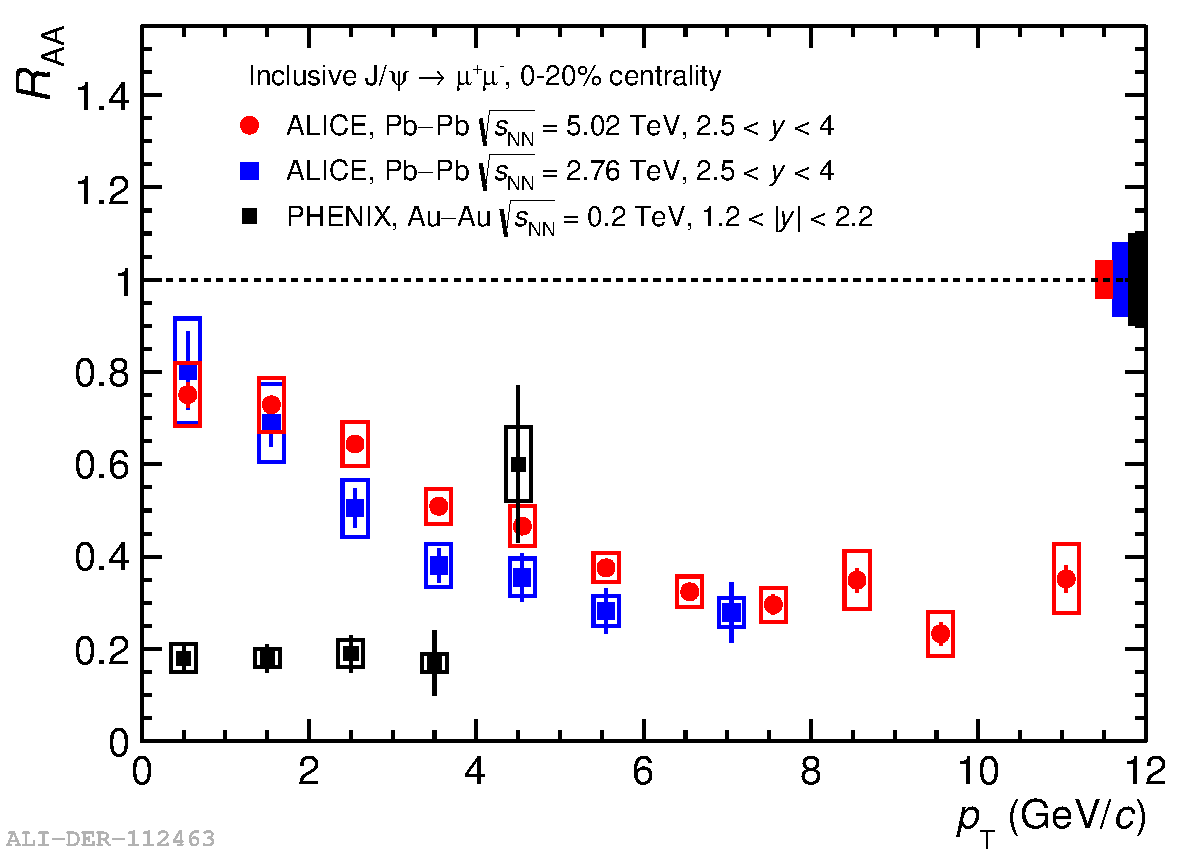
\includegraphics[width=7cm]{FigCap1/RaaJPsiAlicePhenixVsPt.pdf}
  \caption{Centrality (left) and transverse momentum (right) dependence of the J$/\psi$ $\RAA$ measured by ALICE in Pb-Pb collisions at $\sNN = 2.76$ TeV~\cite{Abelev:2013ila} (blue) and at $\sNN = 5.02$ TeV~\cite{Adam:2016rdg} (red) compared to PHENIX~\cite{Adare:2011yf} results Au-Au collisions at $\sNN = 200$ GeV.}
  \label{fig:RaaJPsi}
\end{figure}

\begin{figure}[!ht]
  \centering
  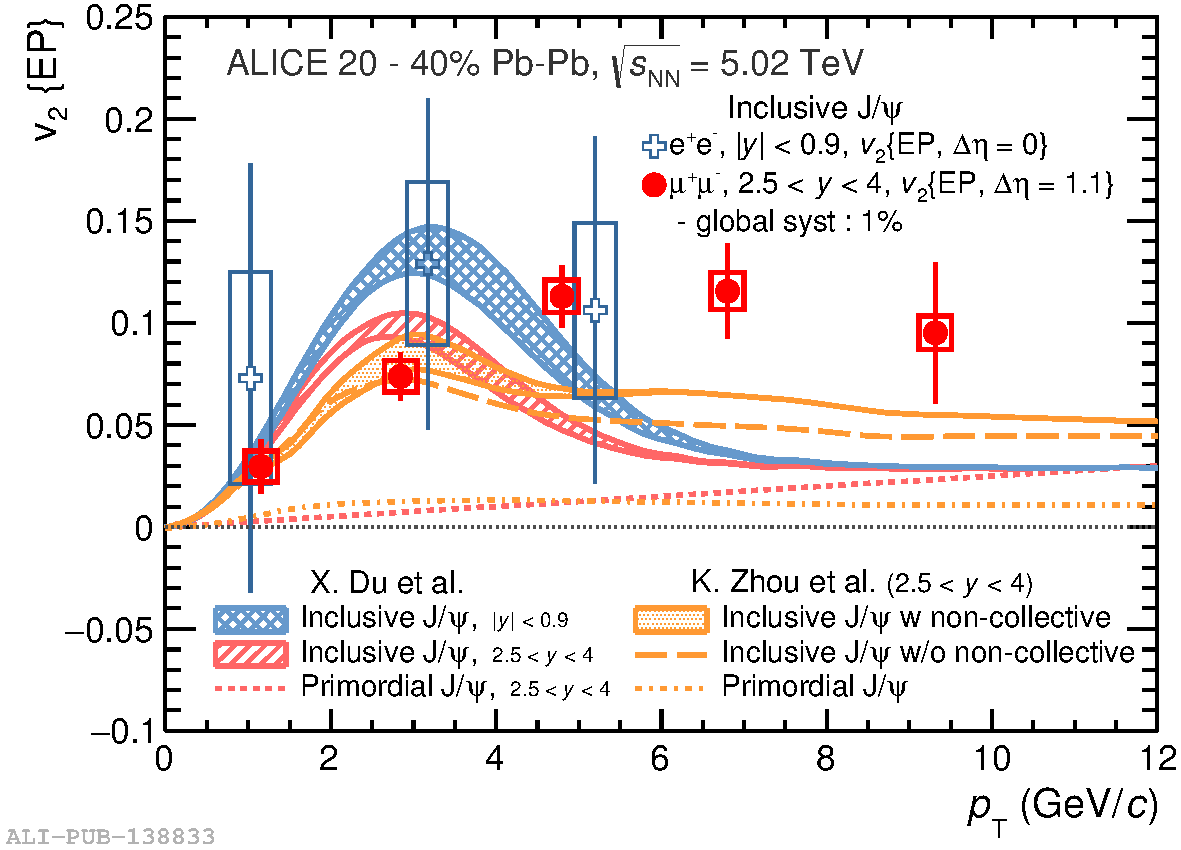
\includegraphics[width=7cm]{FigCap1/JPsiV2Models.pdf}
  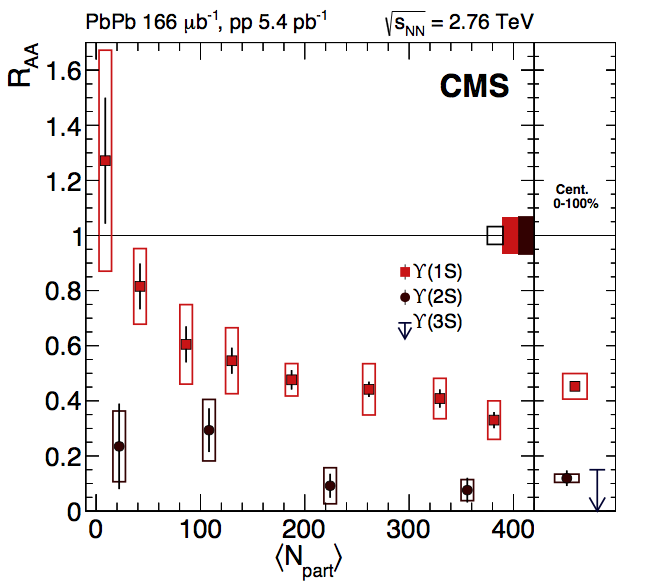
\includegraphics[width=6cm]{FigCap1/RaaUpsilonCMS.png}
  \caption{Left: inclusive J$/\psi$ $v_2(\pt)$ at forward and mid-rapidity for semi-central (20-40\%) Pb-Pb collisions at $\sNN =$ 5.02 TeV~\cite{Acharya:2017tgv}. Calculations from transports model from Refs.~\cite{Du:2015wha} and~\cite{Zhou:2014kka} are also shown. Right: nuclear modification factors of $\Upsilon$(1S) and $\Upsilon$(2S) meson production in Pb-Pb collisions at $\sNN = 2.76$ TeV measured by CMS, as a function of centrality.
The upper limit derived on the nuclear modification factor for $\Upsilon$(3S) is represented with an arrow in the centrality integrated panel on the right~\cite{Khachatryan:2016xxp}. }
  \label{fig:JPsi}
\end{figure}

\subsection{Latest discoveries in small systems}
\label{sec:SmallSystems}
In 2010 CMS discovered first signals of long-range rapidity correlations in 
high-multiplicity pp collisions at $\sqrt{s} = $ 7 TeV~\cite{Khachatryan:2010gv}, a quite unexpected effect 
in small systems. Such correlations
were already observed in Au-Au collisions at RICH~\cite{Alver:2008aa,Alver:2009id,Abelev:2009jv}
and naturally explained in terms of collective expansion of the medium formed in the collisions.
This observation paved the way to searching further signals of collective 
behaviours in small systems. 
The interest in the angular correlations among particles lays in the possibility 
to reveal the underlying mechanisms of particle production. In~\cite{Khachatryan:2010gv}, 
CMS studied the two-dimensional $\Delta \eta$-$\Delta \phi$ correlation 
function, where $\Delta \eta$ is the difference in pseudo-rapidity between 
two particles and $\Delta \phi$ is the difference in their azimuthal angle $\phi$. The $\pt$-inclusive two-particle 
correlation, as a function of $\Delta \eta$ and $\Delta \phi$ is defined as:
\begin{equation}
\label{CorrelationFnc}
R(\Delta \eta,\Delta \phi) = \Big \langle (\langle N \rangle -1) \Big (\frac{S_N(\Delta \eta,\Delta \phi)}{B_N(\Delta \eta,\Delta \phi)} -1\Big )\Big \rangle,
\end{equation}
where (i) $S_N(\Delta \eta,\Delta \phi)$ is the correlation function for the signal distribution,
determined by counting all particle pairs in each event within a multiplicity bin, 
(ii) $B_N(\Delta \eta,\Delta \phi)$ is the correlation function for the background distribution, determined
  by correlating each charged particle of one event with every particle from 
a different event within the same multiplicity bin, (iii) the average is made over all the multiplicity bins of the analysis.
\iffalse
We can define now two correlation functions, the first one, $S_N(\Delta \eta,\Delta \phi)$ for the signal distribution:
\begin{equation}
\label{SignalDistribution}
S_N(\Delta \eta,\Delta \phi) = \frac{1}{N(N-1)}\frac{d^2N^{signal}}{d\Delta \eta d\Delta \phi}
\end{equation}
and the second, $B_N(\Delta \eta,\Delta \phi)$, for the background distribution:
\begin{equation}
\label{BkgDistribution}
B_N(\Delta \eta,\Delta \phi) = \frac{1}{N^2}\frac{d^2N^{mixed}}{d\Delta \eta d\Delta \phi}.
\end{equation}
$S_N(\Delta \eta,\Delta \phi)$ can be determined by counting all particle pairs in each 
event within a multiplicity bin, using the weighting factor $N(N-1)$. $B_N(\Delta \eta,\Delta \phi)$ 
is obtained instead by correlating each charged particle of one event with every particle from 
a different event within the same multiplicity bin. Finally, the $\pt$-inclusive two-particle 
correlation, as a function of $\Delta \eta$ and $\Delta \phi$ is obtained as:
\begin{equation}
\label{CorrelationFnc}
R(\Delta \eta,\Delta \phi) = \Big \langle (\langle N \rangle -1) \Big (\frac{S_N(\Delta \eta,\Delta \phi)}{B_N(\Delta \eta,\Delta \phi)} -1\Big )\Big \rangle,
\end{equation}
where the average is made over all the multiplicity bins of the analysis. 
\fi
By using the ratio of $S_N(\Delta \eta,\Delta \phi)$ and $B_N(\Delta \eta,\Delta \phi)$, 
detector effects such as tracking inefficiencies, non-uniform acceptances, etc, are 
automatically corrected for. In Fig.~\ref{fig:CMSLongRangeRidge_pp7TeV}, $R(\Delta \eta,\Delta \phi)$ 
is plotted for high-multiplicity events ($N_{tracks} > 110$) in pp collisions at $\sqrt{s} = $ 7 TeV, 
selecting tracks with $1 <\pt < 3\; \Gevc$. Several correlation structures are present. 
The narrow peak at $(\Delta \eta, \Delta \phi) \approx (0,0)$ is the contribution 
from jet-like particle production (near-side peak). The broad ridge around $\Delta \phi \approx \pi$ 
is due to the fragmentation of back-to-back jets (away-side ridge). The ridge-like 
structure that appears around $\Delta \phi \approx 0$ was unexpected,
 indeed never observed in two-particle correlations in pp data.
Event generators, such as PYTHIA, did not reproduce the 
 observed structure, that seems to resemble hydrodynamic behaviours of heavy-ion 
 collisions~\cite{Alver:2008aa,Alver:2009id,Abelev:2009jv}, and the physical origin is still not clear.
\begin{figure}[!ht]
  \centering
  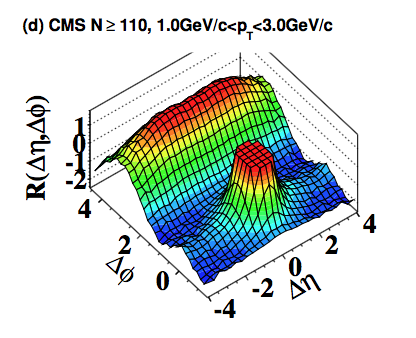
\includegraphics[width=7cm]{FigCap1/CMSLongRangeRidge_pp7TeV.png}
  \caption{Two-particle correlation functions in $\Delta \eta$-$\Delta \phi$ for 7 TeV pp collisions, in high multiplicity events ($N_{trk}>110$), with 1 $< \pt < 3 \,\Gevc$~\cite{Khachatryan:2010gv}.}
  \label{fig:CMSLongRangeRidge_pp7TeV}
\end{figure}
From this first observation, many studies have been done to unravel the nature of the 
long-range near-side peak. Correlations among several produced particles have been explored, 
since this allows to further suppress short-range particle correlations, 
such as jets or resonance decays, in order to further investigate the collective nature 
of the observed azimuthal correlations. One of the most used methods is the 
Q-cumulants method. Following the approach in~\cite{Bilandzic:2010jr}, the 
correlations of two, four and six particles are evaluated as:
\begin{equation}
\label{correlations}
\begin{aligned}
\langle \langle 2 \rangle \rangle &= \langle \langle e^{in(\phi_1 -\phi_2)} \rangle \rangle &\\
\langle \langle 4 \rangle \rangle &= \langle \langle e^{in(\phi_1 + \phi_2 -\phi_3 - \phi_4)} \rangle \rangle &\\
\langle \langle 6 \rangle \rangle &= \langle \langle e^{in(\phi_1 + \phi_2 +\phi_3 - \phi_4- \phi_5- \phi_6))} \rangle \rangle,&
\end{aligned}
\end{equation}
where $\phi_i$ are the azimuthal angles of the correlated particles in an event, $n$ is the harmonic number and $\langle \langle ... \rangle \rangle$ indicates the average over all combinations from all events in a given multiplicity range. The cumulants are obtained as follows:
\begin{equation}
\label{eq:cumulants}
\begin{aligned}
\begin{split}
c_n\{4\} &= \langle \langle 4 \rangle \rangle - 2 \times  \langle \langle 2 \rangle \rangle^2 \\
c_n\{6\} &= \langle \langle 6 \rangle \rangle - 9 \times  \langle \langle 4 \rangle \rangle \langle \langle 2 \rangle \rangle + 12 \times \langle \langle 2 \rangle \rangle^3.
\end{split}
\end{aligned}
\end{equation}
Finally the Fourier harmonics $v_n$ coefficients are obtained from cumulants in Eq.~\ref{eq:cumulants} as:
\begin{equation}
\begin{aligned}
v_n \{4\} = \sqrt[4]{-c_n\{4\}} \\
v_n \{6\} = \sqrt[6]{\frac{1}{4}c_n\{6\}}.
\end{aligned}
\end{equation}
\begin{figure}[!ht]
  \centering
  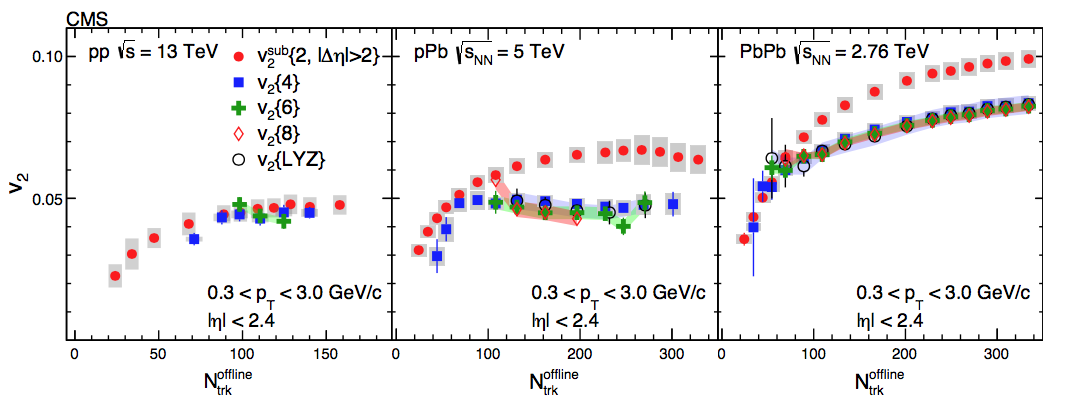
\includegraphics[width=15cm]{FigCap1/v2CumulantsCMS.png}
  \caption{$v_2^{sub} \{2,\, |\Delta \eta| > 2\}$, $v_2 \{4\}$, $v_2 \{6\}$, $v_2 \{8\}$ 
  and $v_2 \{LYZ\}$ as a function of the multiplicity, 
  in the interval $0.3 < \pt < 3\, \Gevc$ and $|\eta| < 2.4$~\cite{Khachatryan:2016txc} measured by CMS, in pp, p-Pb and Pb-Pb collisions.}
  \label{fig:CumulantsCMS}
\end{figure}
In the left panel of Fig.~\ref{fig:CumulantsCMS}, the $v_2 \{4\}$, $v_2 \{6\}$
measured by CMS in pp collisions at $\sqrt{s} = 13$ TeV are shown as a 
function of the particle multiplicity, in the interval $0.3 < \pt < 3 \; \Gevc$ and 
$|\eta| < 2.4$. In the middle and right panels of the same figure, also the $v_2 \{8\}$ and $v_2 \{ {\rm LYZ} \}$ 
(from Lee-Yang zeros method~\cite{Bhalerao:2003yq}) coefficients are shown, for p-Pb and Pb-Pb collisions
at $\sNN = $ 5 TeV and $\sNN = $ 2.76 TeV respectively.
$v_2 \{8\}$ and $v_2 \{ {\rm LYZ} \}$ are less affected by non-flow correlations, 
thus are expected to give the 
cleanest values of the genuine collective flow.
The values of $v_2 \{4\}$, $v_2 \{6\}$ and of $v_2 \{8\}$ and  $v_2 \{ {\rm LYZ} \}$, where present, are compatible among 
them in each of the three colliding systems. This supports the idea 
of a collective behaviour behind the long-range correlations observed in pp 
collisions. In alternative to the classical scenario of position-space
anisotropy that must be transposed into final observed momentum-space anisotropies, other theoretical 
calculations, such as the color glass condensate glasma model~\cite{Schenke:2016ksl}, 
interpret the collective behaviour as due to momentum space-anisotropies. These are
already present before the collision via initial interactions of gluons inside the projectile proton or
nucleus. Besides, in Fig.~\ref{fig:CumulantsCMS} the 
$v_2^{sub} \{2$, $|\Delta \eta| > 2\}$, defined from two-particle 
$\Delta \eta$, $\Delta \phi$ correlation after subtraction of jet correlations from low-multiplicity events, 
is also shown. Some hydrodynamical models interpret the similar magnitude 
of $v_2 \{4\}$ and $v_2^{sub} \{2$, $|\Delta \eta| > 2\}$ in pp collisions as the 
consequence of smaller number of initial fluctuating source than in p-Pb and 
Pb-Pb collisions~\cite{Yan:2013laa}.\\
Recently, ALICE reported about the first observation of strangeness production
 enhancement in high-multiplicity pp collisions~\cite{ALICE:2017jyt}. As 
 anticipated in~\ref{subsec:StrangEnhancSPS}, strangeness enhancement 
 was originally proposed as a signature of the Quark-Gluon Plasma and 
 verified to be even more pronounced for multi-strange baryons. The production 
 of strange hadrons in heavy-ion collisions can be described using a 
 grand-canonical statistical model and does not show a significant dependence 
 on the collision centrality, if one excludes the very peripheral events. For the latter,
  the relative yield of strange particles to pions becomes very similar to what 
  observed in pp and in p-Pb~\cite{Abelev:2013haa,Adam:2015vsf} collisions, and this is understood
  in terms of canonical suppression~\cite{Tounsi:2001ck}. In~\cite{ALICE:2017jyt}, ALICE presented the
   measurement of the production of primary strange ($K^0_S,\; \Lambda,\; \bar{\Lambda}$) 
   and multi-strange ($\Xi^-,\; \Xi^+,\; \Omega^-,\; \Omega^+$) hadrons in pp 
   collisions at $\sqrt{s} = 7$ TeV. Fig.~\ref{fig:StrangenessALICEpp} (left panel) 
   shows the $\pt$-differential yields of 
   $K^0_S,\; \Lambda + \bar{\Lambda},\; \Xi^- + \Xi^+,\; \Omega^- + \Omega^+$ 
   at mid-rapidity, for a selection of classes of events with progressively lower 
   multiplicity, indicated by roman numbers in bracket in the figure. It can be 
   noticed that the $\pt$ spectra become harder as the multiplicity increases, 
   and the hardening becomes stronger with increasing particle mass. This is
    a feature already observed in p-Pb collisions~\cite{Abelev:2013haa} and 
    typically characterizing Pb-Pb collisions, where they are described in terms 
    of relativistic hydrodynamical expansion. A simultaneous fit with the 
    blast-wave model to all $\pt$ spectra in the common highest multiplicity class 
    (I in Fig.~\ref{fig:StrangenessALICEpp} left) and in defined $\pt$ ranges allowed the 
    extraction of the chemical freeze-out temperature $T_{\rm fo} = 163 \pm 10$ 
    MeV and the transverse velocity of the bulk 
    $\langle \beta_{\perp} \rangle = 0.49 \pm 0.02$. The $\pt$ distributions were
     then fitted in their full $\pt$ range using a Tsallis-L\`evy function to obtain the 
     $\pt$-integrated yields. Finally, the right panel of Fig.~\ref{fig:StrangenessALICEpp}
      shows the ratio of $\pt$-integrated hadron yields to the pion yields, as a 
      function of the charged-particle multiplicity, together with the measurements
       in p-Pb ($\sNN = 5.02$ TeV) and Pb-Pb ($\sNN = 2.76$ TeV) collisions. 
       Despite the different energy of the collisions, the ratios show a smooth 
       increase from pp to most central Pb-Pb collisions, with the highest multiplicity 
       points in pp being fully compatible with the magnitude of the enhancement in 
       p-Pb at same multiplicity values or in most peripheral Pb-Pb collisions. At higher multiplicities,
       the ratios in Pb-Pb collisions do not show particular dependence on the collision centrality. This 
       suggests that the mechanism of strangeness enhancement is rather related
        with the characteristics of the final state produced in the collisions, than the
         characteristics of the collision itself. Still, the physical mechanism remains 
         unclear, since the available models fail in reproducing at the same time both
          the ratios in Fig.~\ref{fig:StrangenessALICEpp} and the $\pt$-integrated 
          proton to pion ratios at mid-rapidity~\cite{ALICE:2017jyt}.
\begin{figure}[!ht]
  \centering
  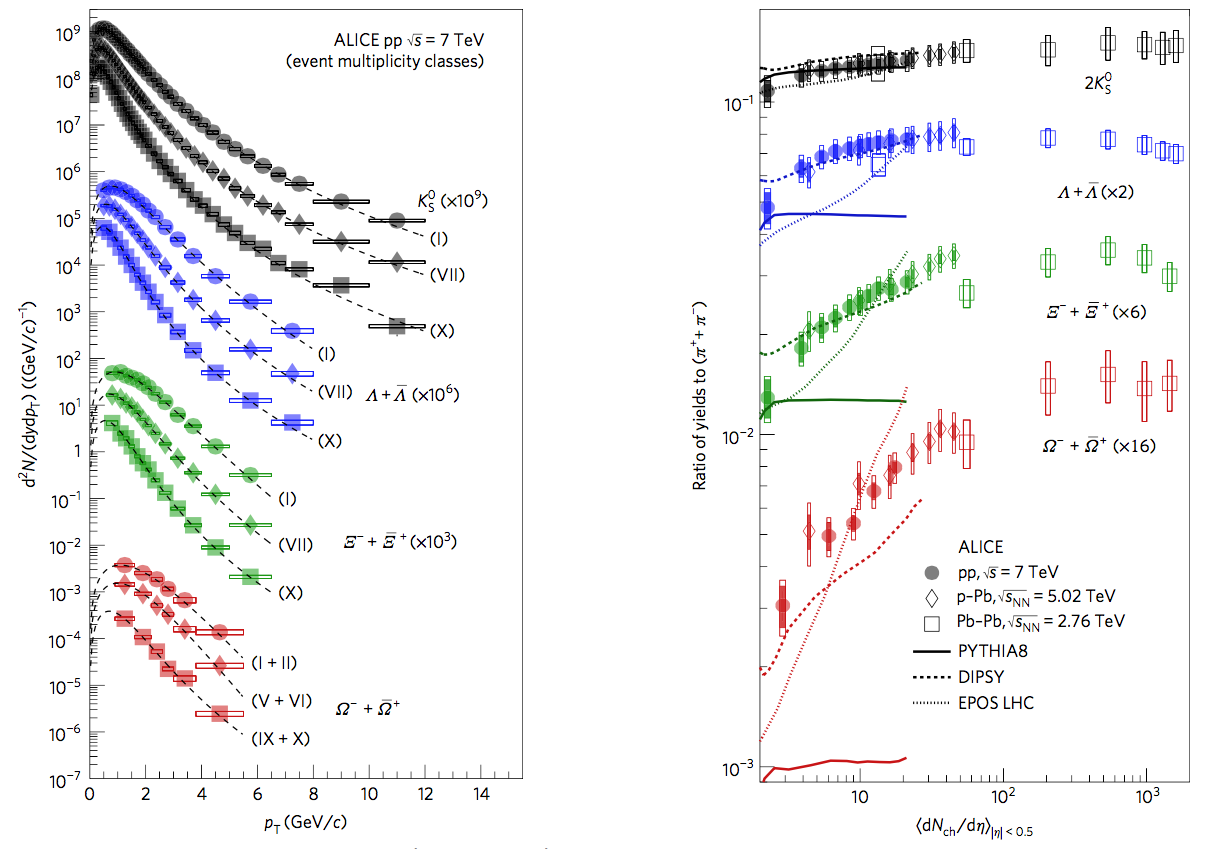
\includegraphics[width=14cm]{FigCap1/StrangenessALICEpp.png}
  \caption{Left: $\pt$-differential yields of $K^0_S,\; \Lambda + \bar{\Lambda}, \Xi^- + \Xi^+,\; \Omega^- + \Omega^+$ at mid-rapidity, for a selection of classes of events with progressively lower multiplicity. The Tsallis-L\`evy fit is shown as dashed line. Right: $\pt$-integrated ratios of $K^0_S,\; \Lambda + \bar{\Lambda},\; \Xi^- + \Xi^+,\; \Omega^- + \Omega^+$ to pion yield ($\pi^- + \pi^+$) as a function of $\langle{\rm d}N_{\rm ch}/{\rm d}\eta \rangle$ at mid-rapidity~\cite{ALICE:2017jyt}.}
  \label{fig:StrangenessALICEpp}
\end{figure}













